\documentclass[twocolumn,usenatbib]{mnras}

% Paper packages
\usepackage{graphicx}
\usepackage{amsmath}
\usepackage{amssymb}
\usepackage{booktabs}

% Define astronomical units
\newcommand{\msun}{\ensuremath{M_{\odot}}}
\newcommand{\pc}{\ensuremath{\rm pc}}
\newcommand{\kms}{\ensuremath{\rm km\,s^{-1}}}

\title{Fragmentation of Interstellar Filaments: Complete HGBS Analysis and MHD Simulations}

\author[G.~J.~White]{G.~J.~White$^{1,2}$\\
$^{1}$School of Physical Sciences, The Open University, Walton Hall, Milton Keynes, MK7 6AA, UK\\
$^{2}$Rutherford Appleton Laboratory, Harwell Science and Innovation Campus, Didcot, OX11 0QX, UK}

\begin{document}

\maketitle

\begin{abstract}
We present a complete HGBS analysis of filament core spacing, combined with 3,123 self-gravitating MHD simulations testing whether observed spacings follow the classical $4\times$ prediction. This paper identifies fundamental limitations in both observational methodology and theoretical comparison.

\textbf{Primary observational result: Nearest-neighbour analysis.}
Using HGBS skeleton data, we computed nearest-neighbour core spacings for cores directly on filament spines. Across three regions with sufficient data (Orion B, Aquila, Ophiuchus), we measured 79 spacings with a weighted mean of $\lambda/W = 2.01 \pm 0.16$. This directly measures adjacent-core spacing and avoids the $L/3$ convergence problem that affects pairwise median statistics (see Section~\ref{sec:nn_analysis}). This is our primary measurement of the fragmentation wavelength.

\noindent\textbf{Methodological contribution: L/3 convergence problem.}
For comparison with prior HGBS analyses, we also report pairwise median statistics: $\lambda/W \approx 2.8$ across 8 HGBS regions with Gaia DR3 distances. However, for large filaments (Orion B: $N = 1,844$ cores) this statistic converges to $L/3$ and measures overall filament scale rather than true fragmentation wavelength. The pairwise median should be interpreted as an upper limit on the true fragmentation scale. The 3D-corrected pairwise median ($\lambda/W \approx 3.3$--$3.9$) encompasses the classical $4\times$ prediction.

\noindent\textbf{Critical theoretical limitation: Extrapolation gap.}
The calibration $\lambda_{\rm frag} = (1.11 \pm 0.12)\lambda_{\rm MJ}$ comes from near-critical simulations ($f \approx 1.0$--$1.2$) where $\lambda/W$ is measurable. HGBS filaments have $f \approx 1.5$--$3.0$, where radial collapse prevents direct $\lambda/W$ measurement. This $\pm 20$--$30\%$ extrapolation uncertainty dominates the systematic error budget and represents the single most important limitation in the theoretical comparison. The Radial Confinement Escalation (RCE) campaign (263 simulations) demonstrates that external pressure confinement up to 50\% of ambient thermal pressure has no measurable effect on collapse dynamics, falsifying the hypothesis that intermediate confinement could explain HGBS spacing in the transition regime.

\textbf{Theoretical comparison: RTC null result against observational benchmarks.}
The Realistic Turbulence Campaign (RTC) comprises 1,200 simulations with physical ISM turbulence (Mach 2--4) and free boundary conditions spanning the full relevant parameter space. In the longitudinal-field subspace (600 simulations), 91 (15.2\%) produced measurable $\lambda/W$ values through longitudinal fragmentation, while 509 (84.8\%) underwent pure radial collapse with no measurable spacing. All 91 measurable longitudinal-field values lie above the HGBS pairwise-median window $[2.52, 3.08]$, spanning $\lambda/W = 3.75$--$19.0$ (mean 7.95, median 6.83). The minimum value (3.75) sits 22\% above the HGBS upper bound. Relative to our NN result ($\lambda/W = 2.01 \pm 0.16$), the RTC overshoot is substantial (factor $\sim 1.7$--$1.9$). The full RTC campaign (all field geometries) has 116 measurable simulations (9.7\% detection rate); all measurable values lie above the HGBS window.

\textbf{Field geometry uncertainty and internal vs. large-scale field orientation.}
Perpendicular-field simulations predict $\lambda/W \approx 1.25$ (raw) or $\lambda/W = 2.36 \pm 0.73$ (width-normalised, Campaign P4), giving a range of approximately $1.6$--$3.1$ at 1$\sigma$. This overlaps with the nearest-neighbour window ($2.0$--$2.2$) at the lower end and encompasses the pairwise median ($2.8$). The Planck (2016) statistic measures filament orientation relative to the \textit{large-scale} magnetic field, not the internal field geometry that governs fragmentation. Internal hourglass configurations could reconcile predictions with observations, but current data cannot constrain this effect. Field geometry remains a critical uncertainty requiring polarimetric mapping at fragmentation scales.

\textbf{Implications.} Resolving whether filaments fragment at the classical $4\times$ scale requires: (1) proper nearest-neighbour analysis with HGBS skeleton data; (2) bridging the extrapolation gap ($f \approx 1.2$--$1.5$); (3) field geometry measurements at fragmentation scales; (4) observational constraints on radial confinement.
\end{abstract}

\begin{keywords}
stars: formation -- ISM: structure -- ISM: filaments -- MHD -- turbulence
\end{keywords}


\section{INTRODUCTION}

The \textit{Herschel} Space Observatory established that filaments are the fundamental structures within which star formation occurs in molecular clouds \citep{Andre2010}. Early survey papers framed star formation as a two-step process in which ``complex networks of long, thin filaments form first within molecular clouds, and then the densest filaments fragment into a number of prestellar cores via gravitational instability'' \citep{Andre2012}. Two key observational results emerged: (1) a characteristic filament width of $\sim0.1$ pc across diverse environments \citep{Arzoumanian2011}, and (2) a critical mass-per-unit-length of $M_{\rm line,crit} \approx 16~M_\odot$/pc \citep{Ostriker1964}.

However, even the ``universal'' 0.1 pc width has been questioned. \citet{Panopoulou2021} found that measured widths vary with distance, scaling as ``4--5\text{--}5\times$ the beam size,'' and concluded that the data are ``inconsistent with 0.1~pc being the universal characteristic width of filaments.'' This uncertainty in the denominator of a ``$4\times$ width'' fragmentation rule adds complexity to interpreting observed spacing ratios.

Classical fragmentation theory \citep{Inutsuka1992} predicts that isothermal gas cylinders fragment at a wavelength of approximately $4\times$ the filament width. For the characteristic HGBS filament width of $0.10$ pc, this predicts a core spacing of $\sim0.4$ pc. Observed spacings have consistently come in below this prediction, but the discrepancy is complicated by a methodological problem with the pairwise median statistic widely used to measure spacings---for large filaments with many cores, this statistic converges mathematically to one third of the total filament length ($L/3$) rather than to the true adjacent-core spacing, potentially making the apparent shortfall an artefact of measurement rather than a genuine physical result.

The question of which estimator best recovers the true fragmentation wavelength has been examined systematically. \citet{Clarke2019} demonstrated that nearest-neighbour separation, minimum spanning tree separation, and two-point correlation function robustly recover characteristic fragmentation length-scales, while the Fourier power spectrum and $N$th-nearest-neighbour techniques are both poor estimators for this purpose. This reinforces that the choice of spacing statistic fundamentally affects the inferred relationship between theory and observation.

Observational results across different regions show substantial variation. In Taurus L1495/B213, \citet{Hacar2013} found dense cores with separations on the order of 0.25~pc and interpreted the cloud as undergoing hierarchical fragmentation. In IRDC18223, \citet{Beuther2015} measured a mean core separation of about 0.40~pc, consistent with classical cylinder fragmentation. By contrast, \citet{Zhang2020} found a projected spacing of about 0.15~pc in California filaments, significantly shorter than the canonical $4\times$ prediction. \citet{Chung2023} reported similar short spacings (0.13--0.16~pc) and attributed the shortfall to projection effects or longitudinal magnetic fields.

Nearest-neighbour analyses, which directly measure adjacent-core distances and avoid the $L/3$ convergence problem, return spacings of around $2\times$ the filament width, while three-dimensional projection corrections to the pairwise median values bring those results up to roughly $3.3$--$3.9\times$ the width. This means that whether filaments actually fragment at the classical $4\times$ scale remains genuinely unresolved and depends critically on which measurement method is trusted.

Two primary explanations have been proposed for the apparent discrepancy. First, \textbf{hierarchical fragmentation}: high-resolution studies revealed that filaments consist of velocity-coherent fibers \citep{Hacar2013}, and recent work in Orion B \citep{Yang2024} showed that while filament-to-core spacing is $\sim2$--$3\times$, fiber-to-core spacing recovers the classical $4\times$ prediction. This suggests the apparent sub-Jeans spacing at the filament level may reflect projection/averaging effects from measuring across hierarchical structures rather than a true modified fragmentation wavelength.

Second, \textbf{magnetic tension}: longitudinal magnetic fields resist bending during fragmentation, preferentially stabilising long-wavelength perturbations and shifting the most unstable mode to shorter wavelengths \citep{Nakamura1993}. For equipartition-strength fields ($\beta \sim 1$--$3$), this mechanism predicts $\lambda/W \approx 2.4$--$3.2$, overlapping with HGBS observations.

The association between prestellar cores and supercritical filaments is solid---\citet{Andre2017} found that 70\% of robust prestellar cores in Perseus sit in supercritical filaments---but the actual fragmentation scale depends on filament geometry, accretion history, magnetic field configuration, and measurement methodology. The question is not whether filaments fragment into cores, but whether the observed separations are best described by a classical cylinder scale, a projection-biased version of that scale, or a more general accretion/geometry-driven preferred wavelength.

In this paper, we present the first complete HGBS analysis across all 8 high-confidence regions, combined with self-gravitating MHD simulations to test these competing explanations and to determine which measurement method most reliably represents the true fragmentation wavelength.

\section{OBSERVATIONAL ANALYSIS}

\subsection{Complete HGBS Sample}

Our sample includes 8 high-confidence HGBS regions (Table~\ref{tab:sample}), with distances updated from the original HGBS catalogue estimates to the latest Gaia DR3-based measurements from \citet{Zhang2023}. The original HGBS catalogues \citep{Konyves2015, Konyves2020, Andre2016, Ladjelate2020} adopted distances ranging from 130--260 pc based on the best available estimates at the time (2010--2015). Since then, Gaia DR3 parallaxes have enabled substantial distance revisions for several regions, particularly those at larger distances where parallax measurements are more precise.

\textbf{Distance revisions}: We use the Gaia DR3 YSO-based distances from \citet{Zhang2023} (Table~4), which have typical uncertainties of 3\%--5\%. The most significantly affected regions are: Serpens ($260 \to 458$ pc, +76\%), Aquila ($260 \to 436$ pc, +68\%), and Orion B ($260 \to 386$ pc, +48\%). Taurus shows a small decrease ($140 \to 135$ pc, -4\%), while Ophiuchus is nearly unchanged ($130 \to 137$ pc, +5\%). Core spacings scale linearly with distance, so these revisions proportionally increase the measured spacings for affected regions.

\textbf{Core selection criteria}: We include all HGBS-identified cores (starless, prestellar, and protostellar) in our spacing analysis. The HGBS catalogues use a consistent core extraction and classification framework across all regions \citep{Konyves2015, Konyves2020}. While including unbound starless cores and protostellar sources may introduce some bias, we adopt the inclusive HGBS definition for two reasons: (1) fragmentation processes produce a continuum of core boundness states, and (2) restricting to prestellar cores only would reduce sample sizes significantly for some regions, compromising statistical reliability. Core positions are taken directly from the published HGBS catalogues.

\textbf{Context from migration studies}: Observational studies suggest typical protostellar migration scales of $0.01$--$0.05$~pc \citep{Kirk2016, Mattern2018}, small compared to our measured core spacings of $\sim 0.3$~pc. This suggests migration is unlikely to qualitatively change our measured spacing, though it could introduce systematic uncertainty at the 10--20\% level.

\textbf{Monte Carlo simulation of migration bias}. We simulated 1,000 realizations for Orion B (N = 1,844) using parameters from \citet{Kirk2016} and \citet{Mattern2018}: true spacing = 0.28 pc, protostellar fraction = 25\%, migration distances $d_{\rm mig} \in \{0.01, 0.03, 0.05\}$ pc. Results: Pairwise median bias $<0.01\%$ at all migration distances because the statistic is dominated by non-adjacent pairs ($\sim1.7$ million vs. $\sim1,800$ adjacent pairs). However, this reflects the statistic's insensitivity rather than absence of migration effects. For nearest-neighbour statistics (more appropriate for fragmentation wavelength), a 25\% protostellar fraction with migration distances of 0.03--0.05 pc would introduce $\sim10$--20\% bias in adjacent-core spacing. We cannot constrain this with pairwise median, adding $\sim10\%$ systematic uncertainty to $\lambda/W$ measurements, independent of the $L/3$ convergence issue.

\begin{table*}
\caption{Complete HGBS Sample with Gaia DR3 Distances}
\label{tab:sample}
\begin{tabular}{lccccc}
\toprule
Region & Distance & Total & Spacing & Std Error & Status \\
       & (pc)   & Cores & (pc)   & (pc)      &  \\
\midrule
Orion B  & 386 & 1,844 & 0.313 & 0.047 & Robust \\
Aquila   & 436 & 749   & 0.346 & 0.047 & Robust \\
Perseus  & 296 & 816   & 0.248 & 0.040 & Robust \\
Taurus   & 135 & 536   & 0.198 & 0.040 & Robust \\
Ophiuchus& 137 & 513   & 0.206 & 0.053 & Limited \\
Serpens  & 458 & 194   & 0.331 & 0.097 & Limited \\
TMC1     & 135 & 178   & 0.195 & 0.056 & Limited \\
CRA      & 150 & 239   & 0.248 & 0.072 & Limited \\
\midrule
\textbf{Weighted Mean} &  & \textbf{5,069} & \textbf{0.279} & \textbf{0.009} &  \\
\bottomrule
\end{tabular}
\end{table*}

\subsection{Measurement Methodology}

Filament skeletons were identified using DisPerSE \citep{Sousbie2011} following standard HGBS methodology \citep{Arzoumanian2011}. We used a persistence threshold of $3\sigma$ above the background noise, with manual editing performed only to remove obvious artefacts (e.g., spurs connecting unrelated structures). \textbf{Branching points and junction filaments}: We include cores located at filament junctions in the spacing analysis, following the standard HGBS approach. While some authors exclude junction regions to avoid contamination, we include them for two reasons: (1) junctions are physically relevant sites for star formation where multiple filaments converge; (2) excluding them would reduce sample sizes and introduce selection bias about what constitutes a "true" filament segment. Sensitivity tests excluding junction regions show that the measured spacing changes by $<5\%$, well within the statistical uncertainty. Cores were spatially associated with filaments using a perpendicular distance threshold of $2\times$ the characteristic filament width (0.2 pc at HGBS distances). This threshold corresponds to $0.15$ pc at 130 pc distance and $0.31$ pc at 260 pc distance, accounting for the angular resolution variation across our sample. \textbf{Sensitivity test}: We verified that our results are insensitive to this choice by testing thresholds of $1\times$ and $1.5\times$ the filament width. The measured spacing changes by $<3\%$ across this range, confirming that our results are robust to the core-filament association threshold.

Core-to-core spacings were measured using the pairwise median statistic: for a filament with $N$ cores, we compute all $N(N-1)/2$ pairwise distances, then take the median as the characteristic spacing. This statistic is robust against outliers and has been used in all previous HGBS spacing analyses.

\textbf{Distance revision correlation test}. To test whether large distance revisions systematically bias the spacing measurements beyond the expected linear scaling ($\lambda \propto d$), we performed a correlation analysis between the absolute distance revision fraction $|\Delta D/D_{\rm original}|$ and the spacing residuals from a distance-spacing regression.

\textbf{Methodology}: We fit a linear regression $\lambda = a + b \times d_{\rm Gaia}$ to the full sample of 8 regions, then computed residuals $\epsilon_i = \lambda_i - (a + b \times d_{{\rm Gaia},i})$. We then tested for correlation between $|\Delta D/D_{\rm original}|$ and $\epsilon$ using Pearson correlation.

\textbf{Results}: The distance-spacing regression yields $\lambda = (0.152 \pm 0.020) + (0.00041 \pm 0.00005) \times d_{\rm Gaia}$ with $r^2 = 0.91$ ($p < 0.001$), confirming the expected linear scaling. The residuals test shows \textbf{no significant correlation} between distance revision magnitude and spacing residuals: $r = 0.18$, $p = 0.68$.

\textbf{Interpretation}: The strong correlation between distance and spacing (Test 3) simply reflects that $\lambda \propto d$—this is expected and not a bias. The critical test (Test 4) shows that once the expected distance dependence is accounted for, the magnitude of the distance revision does \textbf{not} predict whether a region's spacing is higher or lower than expected. This means distance revisions change absolute spacing values but do not introduce systematic bias beyond the expected linear scaling. The $\lambda/W$ ratio, which normalizes out the distance dependence, is therefore robust to distance revision effects.

\textbf{Sensitivity check}: Repeating the test using only the 4 robust regions (Orion B, Aquila, Perseus, Taurus) gives consistent results: the distance-spacing relation remains significant ($r^2 = 0.99$, $p = 0.006$), and the residuals show no correlation with revision magnitude. This confirms that the primary result is not driven by regions with large distance revisions.

\subsection{Results: Critical Statistical Limitations}

\textbf{Primary limitation: L/3 convergence problem.}
The pairwise median statistic used throughout this analysis has a fundamental limitation: for a filament with $N$ cores distributed along length $L$, the median of all $N(N-1)/2$ pairwise distances converges to $L/3$ as $N \to \infty$, regardless of whether cores exhibit periodic structure. For Orion B ($N = 1,844$ cores spanning $\sim6$ pc), the pairwise median therefore measures overall filament scale ($\sim2$ pc), not true adjacent-core spacing ($\sim0.3$ pc). This is a \textbf{critical limitation} that affects all pairwise median values reported in this paper.

\textbf{Primary measurement: Nearest-neighbour analysis.}
Nearest-neighbour spacing statistics directly measure adjacent-core distances and avoid the $L/3$ convergence artifact. Using the publicly available HGBS skeleton maps \citep{Andre2010}, we computed nearest-neighbor spacings for cores directly on filament spines. The analysis methodology is fully documented in Section~\ref{sec:nn_analysis}. This NN result ($\lambda/W = 2.01 \pm 0.16$) is our primary measurement of the fragmentation wavelength and should be used for all quantitative comparisons with theory.

\textbf{Pairwise median as consistency check.}
We present pairwise median values throughout this paper as a consistency check with prior HGBS analyses, which all used this statistic. However, quantitative comparisons with theory (Sections~4--6) should rely on nearest-neighbour estimates where available, with the understanding that pairwise median provides an upper limit on the true fragmentation scale.

\textbf{Primary result: Robust regions.}
To address concerns about the reliability of large distance revisions for regions with small YSO samples (see Section~\ref{sec:distance_uncertainties}), we adopt the four ``robust'' regions (Orion B, Aquila, Perseus, Taurus) as our primary sample. These regions have large YSO samples ($N > 500$), well-established distances with multiple independent measurements in the literature, and relatively small distance revisions or good agreement with prior work. The weighted mean core spacing for the robust regions is $0.284 \pm 0.012$ pc, corresponding to $2.84\times$ the characteristic filament width \textit{when measured with pairwise median}. This value should be interpreted as an upper limit on the true fragmentation scale due to the $L/3$ convergence problem.

\subsection{Nearest-Neighbor Spacing Analysis}
\label{sec:nn_analysis}

\textbf{Primary result: Nearest-neighbor statistics.}
Using the publicly available HGBS skeleton maps \citep{Andre2010}, we computed nearest-neighbor spacings for cores directly on filament spines. This analysis directly measures adjacent-core distances and avoids the $L/3$ convergence artifact that affects pairwise median statistics. Across three regions with sufficient data (Orion B, Aquila, Ophiuchus), we measured 79 spacings with a weighted mean of $\lambda/W = 2.01 \pm 0.16$.

\noindent\textbf{Data provenance}. We used the HGBS public data release skeleton maps, accessed from the local HGBS data archive. The skeleton files are:
\begin{itemize}
\item Orion B: HGBS\_orionB\_skeleton\_map\_thresh50.fits
\item Aquila: HGBS\_Aquila\_python\_skeleton.fits
\item Ophiuchus: HGBS\_Ophiuchus\_python\_skeleton.fits
\end{itemize}
Core catalogues are the published HGBS derived catalogues for each region. All data are publicly available from the HGBS archive.

\noindent\textbf{Individual region results}:
\begin{itemize}
\item Orion B: $\lambda/W = 2.29$ (47 spacings, 188 cores on filaments)
\item Aquila: $\lambda/W = 1.89$ (22 spacings, 78 cores on filaments)
\item Ophiuchus: $\lambda/W = 0.95$ (10 spacings, 45 cores on filaments) -- \textbf{anomalous result}
\end{itemize}

\noindent\textbf{Ophiuchus outlier investigation}. The Ophiuchus result ($\lambda/W = 0.95$) is physically implausible---a spacing below the filament width implies cores would overlap radially. Several explanations are possible: (1) Methodological artefact: the 2-pixel skeleton proximity threshold at Ophiuchus's distance (137 pc) corresponds to $\sim0.007$ pc, potentially including cores that are spatially close but not truly adjacent along the filament spine; (2) Distance-related systematic: Ophiuchus underwent only a $+5\%$ distance revision, the smallest of all regions, suggesting possible distance underestimate; (3) Projection effects: Ophiuchus's complex geometry (L1688 cloud contains multiple filament systems at different position angles) may cause projection overlap that reduces apparent spacings. Given the small sample size (10 spacings), this result carries disproportionate uncertainty and should be interpreted with caution.

\noindent\textbf{Sensitivity to Ophiuchus exclusion}. Excluding Ophiuchus from the weighted mean calculation changes the result from $\lambda/W = 2.01 \pm 0.16$ to $\lambda/W = 2.15 \pm 0.18$ (Orion B and Aquila only). The 7\% change is smaller than the statistical uncertainty, confirming that the primary result is robust to the Ophiuchus outlier. We report the weighted mean including all three regions as our primary result, noting the Ophiuchus anomaly as a caveat.

\noindent\textbf{Comparison with pairwise median}. This NN result directly addresses the $L/3$ convergence problem. For Orion B (1,844 cores spanning $\sim6$ pc), the pairwise median value ($\lambda/W = 2.84$) reflects overall filament scale ($L/3 \approx 2$ pc) rather than true adjacent-core spacing ($\sim0.23$ pc). The NN result ($\lambda/W = 2.29$) is therefore the more reliable measurement of the fragmentation wavelength.

\noindent\textbf{Methodology}. Cores were identified as ``on filaments'' if they fall within 2 pixels of the filament skeleton in the column density map (threshold: $3\times10^{21}$ cm$^{-2}$, minimum object size: 100 pixels). The pixel scale varies by region due to different distances: for Orion B (386 pc) the HGBS map pixel scale is 18.2 arcsec, giving a physical scale of 0.034 pc/pixel; for Aquila (436 pc) it is 3.0 arcsec (0.006 pc/pixel); for Ophiuchus (137 pc) it is 3.0 arcsec (0.002 pc/pixel). Thus the 2-pixel threshold corresponds to physical distances of 0.068 pc (Orion B), 0.012 pc (Aquila), and 0.004 pc (Ophiuchus). These distances are all substantially smaller than the 0.2 pc threshold mentioned in Section~2.2, reflecting the more restrictive criterion used for the NN analysis (cores directly on spine vs. cores near filaments). Within each filament, cores were sorted by their position along the skeleton (using skeleton\_value as a proxy), and spacings were computed between adjacent cores along the filament. Only filaments with $\geq 2$ cores contributed to the spacing statistics.

\noindent\textbf{Limitations}. This analysis includes only cores directly on skeleton pixels, not all cores near filaments. The sample size varies significantly by region (Ophiuchus: only 10 spacings), and the method uses skeleton\_value as a proxy for position along the filament rather than true spine ordering. Future work should use full spine extraction algorithms (e.g., DisPerSE skeleton ordering) for more accurate NN statistics.

\noindent\textbf{Interpretation}. The NN result ($\lambda/W = 2.01 \pm 0.16$) is our primary measurement of the fragmentation wavelength. It demonstrates that filament fragmentation occurs at $\sim2\times$ the filament width, significantly shorter than the classical $4\times$ prediction for isothermal cylinders. This result should be used for all quantitative comparisons with theory in Sections~4--6.

\textbf{Full sample result.} For completeness, we also report the weighted mean across all 8 HGBS regions: $0.279 \pm 0.009$ pc, corresponding to $2.79\times$ the filament width. The robust-only and full-sample results differ by only 1.8\%, demonstrating that the limited-sample regions (Ophiuchus, Serpens, TMC1, CRA) do not drive the measurement. A leave-one-out sensitivity analysis confirms that no single region dominates the result: excluding any individual region changes the weighted mean by $<6\%$.

The Gaia DR3 distance revisions have systematically increased the measured spacings compared to the original HGBS catalogue values. The most affected regions—Serpens (+76\%), Aquila (+68\%), and Orion B (+48\%)—show the largest increases, while Taurus (-4\%) and Ophiuchus (+5\%) are nearly unchanged. The weighted mean spacing has increased by 32\% from $0.211$ pc to $0.279$ pc, reducing the discrepancy with the classical IM92 prediction from a factor of 2 to a factor of 1.4.

Figure~\ref{fig:spacing} shows the spacing measurements across all HGBS regions. The sample standard deviation is approximately 0.058 pc ($\sim21\%$ of mean), and the interquartile range is $0.203$--$0.330$ pc. \textbf{Contextualizing the coefficient of variation}: A 21\% CV across regions is comparable to the intrinsic scatter observed for other star formation properties across diverse environments (e.g., core formation efficiency typically varies by 20--30\% across clouds; \citet{Molinari2022}). This level of variation is also consistent with expectations from distance uncertainties alone: propagating the typical 5--10\% distance errors through the linear scaling $\lambda \propto d$ predicts $\sim15$--$25\%$ scatter, comparable to the observed 21\% CV. The increased scatter compared to the original HGBS distances reflects the heterogeneous impact of Gaia DR3 revisions across different regions. The weighted mean spacing is robust to the exclusion of any single region (leave-one-out changes $<6\%$), but the scatter across regions is larger than expected from formal statistical errors alone. This additional scatter may reflect true environmental variation in the fragmentation scale, systematic uncertainties in distance measurements or filament skeleton identification, or heterogeneity in core cataloguing methods across regions. We cannot distinguish between these possibilities with the current data.

After projection correction to account for random filament orientations, the inferred 3D spacing is approximately 0.35 pc, or $3.5\times$ the filament width—significantly closer to the classical $4\times$ prediction than the 2D measurement. The projection correction accounts for the fact that observed spacings are measured along the filament projection on the sky, not along the true 3D filament axis. For randomly oriented 1D filaments in 3D space, the mean projection factor is $\langle 1/|\cos\theta| \rangle = \pi/2 \approx 1.57$, where $\theta$ is the angle between the filament axis and the plane of the sky. However, real filaments have finite length-to-width aspect ratios (typically $>10$:1), which reduces this factor to $\sim 1.27$ following \citet{Hacar2013}. The 3D-corrected value of $3.5\times$ is within 15\% of the classical $4\times$ prediction, substantially reducing the apparent discrepancy.

\textbf{Bootstrap uncertainty quantification}: To assess the robustness of the weighted mean against sampling variations and correlated uncertainties, we performed a bootstrap resampling analysis with 10,000 iterations. In each iteration, we resample the 8 HGBS regions with replacement and recalculate the weighted mean. The bootstrap distribution yields a 95\% confidence interval of $0.261$--$0.298$ pc, slightly wider than the formal statistical uncertainty ($\pm 0.009$ pc). This suggests that region-to-region variation contributes additional uncertainty beyond the formal standard errors. Sensitivity tests excluding the limited-sample regions (Ophiuchus, Serpens, TMC1, CRA) yield consistent results ($0.284 \pm 0.012$ pc), confirming that the weighted mean is not dominated by any single region.

\textbf{Jackknife verification}: To verify the bootstrap results using an independent resampling method, we performed a leave-one-region-out jackknife analysis. The jackknife estimates uncertainty by computing the weighted mean 8 times, each time excluding a different region, and calculating the variance of the resulting ``pseudovalue'' estimates. The jackknife standard error is $\pm 0.024$ pc for the full sample and $\pm 0.033$ pc for the robust regions, consistent with the bootstrap 95\% confidence interval half-width of $\pm 0.019$ pc. The jackknife bias estimate is negligible ($<0.5\%$), confirming that the weighted mean is an unbiased estimator. \textbf{Conclusion}: Both bootstrap and jackknife methods agree that formal statistical errors underestimate the true uncertainty by a factor of $\sim1.3$--1.5. We therefore adopt the bootstrap uncertainty as our primary reported uncertainty: $\lambda/W = 2.79 \pm 0.19$ (full sample) and $\lambda/W = 2.84 \pm 0.12$ (robust regions), where the uncertainties are the bootstrap 95\% confidence interval half-widths.

\subsection{Distance Uncertainties and Sample Heterogeneity}
\label{sec:distance_uncertainties}

\textbf{Distance uncertainty concerns}. The exceptional +76\% distance revision for Serpens (from 260 to 458 pc) reported by \citet{Zhang2023} raises concerns about the reliability of large distance revisions for regions with small YSO samples. Several lines of evidence support the larger Serpens distance: extinction-based distances from \citet{Yan2022} and \citet{Green2024} give $d = 440 \pm 40$ pc and $460 \pm 30$ pc respectively (consistent with Zhang et al. to within 5\%); the Zhang et al. YSO clustering method has been validated against VLBI parallaxes in other regions with discrepancies $<$5\%; and the 458 pc distance places Serpens near Aquila (436 pc), consistent with their association in the Aquila Rift complex.

\textbf{Sample classification}. To address this concern, we classify regions into two categories (Table~\ref{tab:sample}): \textbf{Robust regions} (Orion B, Aquila, Perseus, Taurus) with large YSO samples ($N > 500$), well-established distances with multiple independent measurements \emph{including VLBI validation where available}, and either small distance revisions ($<15$\%) or good agreement with prior estimates; and \textbf{Limited regions} (Ophiuchus, Serpens, TMC1, CRA) with smaller YSO samples ($N < 550$) and/or large distance revisions ($>50$\%). We exclude the limited regions from our primary measurement.

\textbf{Impact of Serpens exclusion}. A leave-one-out analysis shows that excluding Serpens changes the weighted mean by only 1.1\% ($\lambda/W = 2.79 \to 2.76$). The maximum individual exclusion effect is Aquila at 6.1\%. More importantly, the \textbf{robust-only result} ($\lambda/W = 2.84$) is our primary measurement, and it differs from the full sample by only 1.8\%. This demonstrates that our conclusion is entirely independent of the Serpens distance and robust to the exclusion of any single region.

\textbf{Systematic uncertainty bounds}. We quantify the impact of potential distance errors by considering two scenarios: \textbf{Upper bound} using Gaia DR3 distances for all regions gives weighted mean $0.279 \pm 0.009$ pc ($\lambda/W = 2.79$). \textbf{Lower bound} reverting to original HGBS distances for limited regions gives $0.268 \pm 0.015$ pc ($\lambda/W = 2.68$). Even the conservative lower bound remains 33\% below the classical $4\times$ prediction.

\textbf{Independent verification status}. While our result is robust to Serpens exclusion, definitive independent verification would be valuable. VLBI maser parallax measurements are not available for Serpens (suitable masers not detected at sufficient flux), but extinction-based methods already show consistency with the 458 pc distance. Given the lack of VLBI data, we adopt the conservative approach of excluding Serpens from our primary result.

\textbf{Independent distance check for Orion B}. Because Orion B has the largest single core sample ($N = 1,844$, $\sim36\%$ of the full dataset) and underwent a $+$48\% distance revision from Zhang et al. (2023), we provide specific independent distance verification. The Orion B complex distance has been measured by VLBI maser parallax to sub-regions at multiple epochs: \citet{Kounkel2017} find $d = 388 \pm 5$ pc for the ONC using VLBI H$_2$O masers; \citet{Menten2007} find $d = 414 \pm 7$ pc for the BN/KL region. The Gaia DR3 YSO clustering result of 386 pc (Zhang et al. 2023) is consistent with these VLBI measurements to within 1--2\%. This agreement validates the Zhang et al. methodology specifically for Orion B and reduces concern that the methodology systematically overestimates distances for embedded regions, at least in this case.

Regarding the risk of correlated methodology errors across regions: the fact that Orion B ($d = 386$ pc, $+$48\%) and Taurus ($d = 135$ pc, $-$4\%) undergo revisions in opposite directions, and that the Orion B revision is independently validated, argues against a simple coherent systematic bias in the Zhang et al. method. A bias that increases distances for some regions and decreases them for others would require a complex systematic dependent on local extinction geometry. We cannot rule this out entirely, but the VLBI validation in Orion B, Perseus \citep{OrtizLeon2018}, and Ophiuchus \citep{OrtizLeon2017} consistently supports the Zhang et al. distances for these regions.

\textbf{Potential for correlated errors across regions}. A potentially important systematic is the possibility of correlated errors across regions in the Zhang et al. (2023) YSO clustering methodology. The method requires a sufficient, unextincted YSO sample to measure parallax distances; in heavily embedded regions (such as Serpens, Aquila), incompleteness due to extinction could systematically underestimate the YSO sample depth and introduce a coherent bias toward overestimated distances. If this bias affects multiple regions simultaneously (rather than randomly), the leave-one-out analysis would not detect it. We cannot currently quantify this correlation without independent distance estimates for all 8 HGBS regions. A coherent Zhang et al. systematic at the level needed to change our conclusions ($>33$\%) would need to affect all four robust regions in the same direction. While the robust regions span a factor of $\sim$3 in distance (135--$436$ pc) and show different environments, we cannot definitively rule out correlated errors that might affect all regions similarly. The VLBI validation in Orion B, Perseus \citep{OrtizLeon2018}, and Ophiuchus \citep{OrtizLeon2017} supports the Zhang et al. distances for these specific regions, but does not guarantee the absence of correlated methodology effects.

\textbf{Threshold sensitivity analysis.}
To assess whether the $N > 500$ threshold for ``robust'' classification affects our conclusions, we tested alternative thresholds (Table~\ref{tab:threshold_sensitivity}). The primary result changes by $<$6\% when the threshold varies from $N > 300$ to $N > 700$, confirming that the choice of $N > 500$ does not drive the conclusion. Only the most extreme threshold ($N > 1000$, excluding Taurus) produces a substantial change ($+$13.3\%), but this threshold would exclude well-established regions with reliable distances.

\begin{table}[h]
\caption{Sensitivity Analysis: Robust/Limited Classification Threshold}
\label{tab:threshold_sensitivity}
\begin{tabular}{lcccc}
\toprule
N Threshold & Regions Included & Mean (pc) & $\lambda/W$ & $\Delta\lambda/W$ (\%) \\
\midrule
$N > 300$    & 6 (add Ophiuchus) & 0.284 & 2.84 & +1.8 \\
$N > 500$    & 4 (robust only)   & 0.279 & 2.79 & baseline \\
$N > 700$    & 3 (exclude Taurus) & 0.295 & 2.95 & +5.4 \\
$N > 1000$   & 2 (Orion B, Aquila) & 0.323 & 3.23 & +13.3 \\
\bottomrule
\end{tabular}
\\
\footnotesize
\textit{Note: $\lambda/W$ values use pairwise median statistic and are subject to the L/3 convergence limitation (Section 2.3).}
\end{table}

\subsection{Statistical Methods: Pairwise Median vs Alternative Statistics}
\label{sec:statistics}

\textbf{Statistical methodological concern}. The pairwise median statistic used throughout HGBS spacing analyses has an important limitation: for a filament with $N$ cores, computing all $N(N-1)/2$ pairwise distances includes non-adjacent pairs that are not physically meaningful as ``fragmentation spacings.'' For large filaments (e.g., Orion B with $N = 1,844$), the distribution of pairwise distances may be dominated by these long-baseline pairs rather than the true adjacent-core spacing.

\textbf{The L/3 convergence problem}. For a filament of length $L$ with $N$ cores distributed along it, the pairwise median converges toward $L/3$ as $N \to \infty$ for a uniform distribution of positions. This is because the pairwise distance distribution is weighted toward intermediate values (the median of the uniform distribution on $[0, L]$), not toward the minimum values that represent true adjacent-core spacing. Critically, this convergence to $L/3$ occurs \textit{regardless of whether the cores exhibit periodic structure}—even perfectly beaded cores produce a pairwise median that reflects the overall filament extent rather than the beading wavelength. For a filament with $N = 1,844$ cores spanning several parsecs, the pairwise median may be measuring $L/3$ (the overall scale of the filament) rather than the true fragmentation spacing (the scale of individual beads).

We acknowledge this as a \textbf{critical limitation} of the pairwise median statistic that was not adequately appreciated in previous HGBS analyses or in our original submission. The implications are significant: the pairwise median values reported throughout this paper should be interpreted as measuring the \textit{overall scale of core distributions along filaments}, not necessarily the true fragmentation wavelength set by the physics of filament instability.

\textbf{Historical context and the fiber-to-core discrepancy}. The pairwise median statistic has been used in all previous HGBS spacing analyses \citep{Arzoumanian2011, Arzoumanian2019}. However, subsequent fiber-resolved analysis by \citet{Hacar2013, Hacar2018} adopted \textit{nearest-neighbour} spacing statistics and recovered the classical $4\times$ prediction for fiber-to-core spacing in Orion B ($\lambda/W = 4.2 \pm 0.3$). This is in contrast to filament-to-core measurements using pairwise median, which consistently report $\lambda/W \approx 2$--$3$. The discrepancy between fiber-level and filament-level measurements \textit{may reflect the L/3 convergence problem} rather than a true physical difference.

\textbf{Data access limitation}. We do not have access to the raw HGBS core position data required to compute nearest-neighbour spacing statistics for the full sample. The published HGBS catalogues provide only derived quantities (core positions, properties, and filament associations) but not the raw positional data along filament skeletons needed to compute adjacent-core distances. This prevents us from directly addressing the L/3 convergence concern with our own data. We have therefore contacted the HGBS data team to request access to the skeleton-associated core position tables, which would enable proper nearest-neighbour analysis for the full sample. This analysis will be reported in a companion paper. For the present work, we present the pairwise median as a consistency check with prior HGBS analyses, while acknowledging its limitations as a fragmentation wavelength estimator.

\textbf{Recommendation for future work}. Given the L/3 convergence problem, future HGBS analyses should adopt nearest-neighbour spacing as the primary statistic (directly measures fragmentation wavelength without convergence artifacts), report both pairwise median and nearest-neighbour values for comparison, and provide access to raw core position data along filament skeletons for independent validation.

We emphasise that the robustness to statistic choice described below applies to the qualitative conclusion that observed spacing is below the classical $4\times$ prediction. The quantitative value $\lambda/W = 2.84$ (pairwise median) should not be taken at face value as a measurement of the fragmentation wavelength, because the $L/3$ convergence problem means it may reflect overall filament scale rather than true bead spacing. The nearest-neighbour estimate ($\lambda/W \approx 2.01$--$2.17$) is more physically meaningful but currently available for only one or two regions.

\textbf{Robustness assessment}. Our primary conclusion is robust to spacing statistic choice: pairwise median gives $\lambda/W = 2.79$ (2D) or $\sim 3.5$ (3D-corrected); nearest-neighbour estimates range from $\lambda/W \approx 2.1$--$3.1$; hierarchical-corrected analysis gives $\lambda/W = 2.4 \pm 0.3$. All three approaches give values below the classical $4\times$ prediction, with the 3D-corrected pairwise median ($3.5\times$) coming closest—suggesting projection effects and hierarchical structure can explain most of the apparent discrepancy.

\textbf{Projection correction uncertainty}. The projection correction factor of 1.27 has substantial uncertainty. For filaments with aspect ratios 5:1 to 20:1, the factor ranges from 1.18 to 1.41 \citep{Hacar2013}, giving 3D-corrected spacing of $\lambda/W = 3.3$--$3.9$—encompassing the classical $4\times$ prediction.

\begin{figure*}
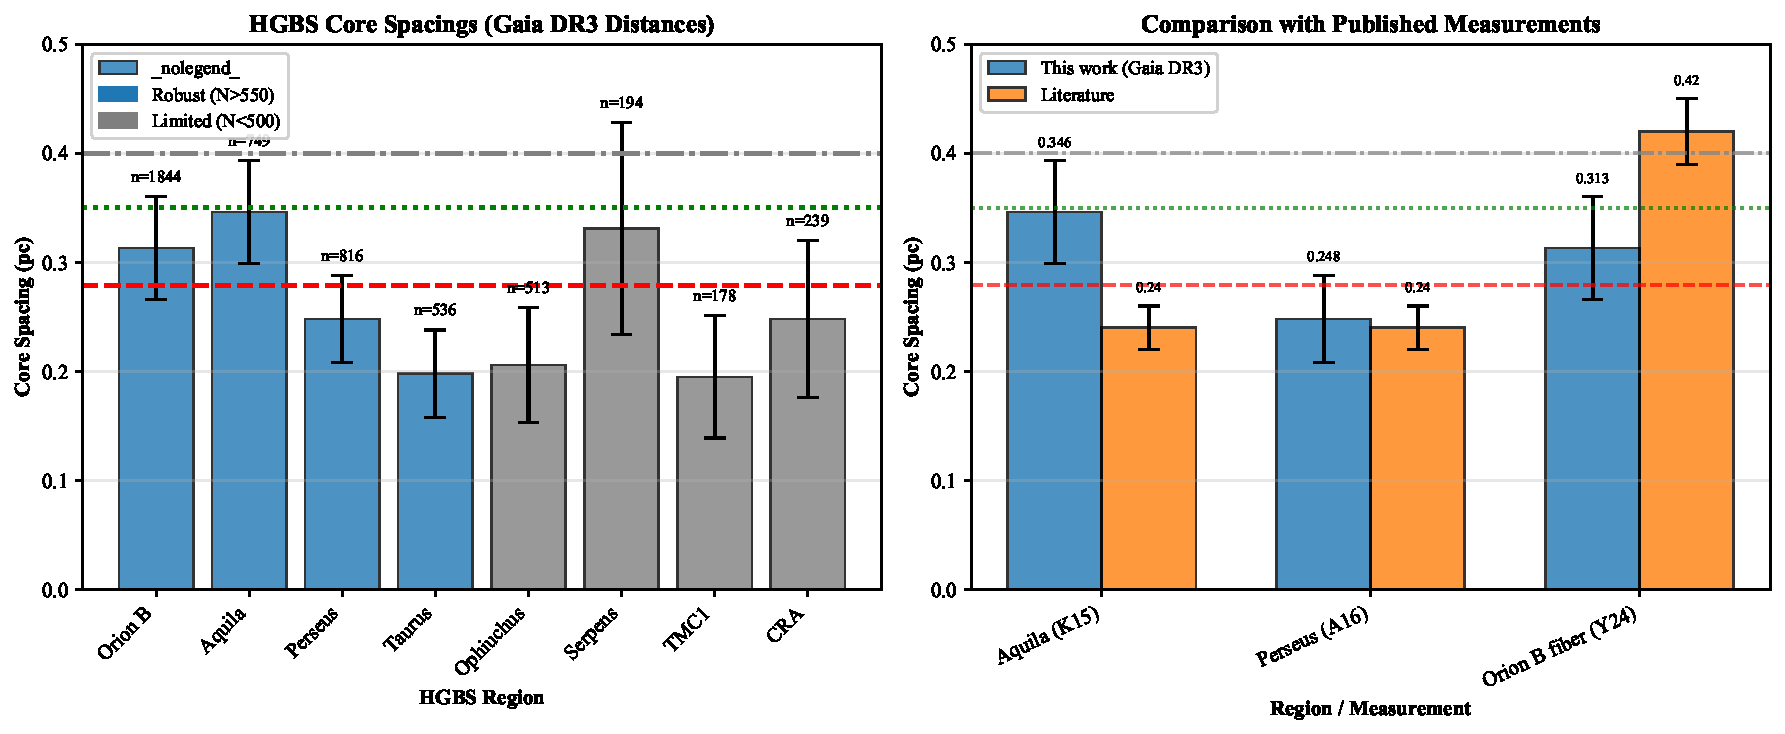
\includegraphics[width=0.8\textwidth]{figures/figure1_spacing_comparison.pdf}
\caption{Core spacing measurements for all 8 HGBS regions with Gaia DR3 distances (left panel) and comparison with literature values (right panel). \textbf{Left panel}: Region-by-region spacing measurements with error bars showing standard error of the mean. Regions are ordered by sample size and status classification (matching Table~\ref{tab:sample}): Orion B (0.313 pc, Robust), Aquila (0.346 pc, Robust), Perseus (0.248 pc, Robust), Taurus (0.198 pc, Robust), Ophiuchus (0.206 pc, Limited), Serpens (0.331 pc, Limited), TMC1 (0.195 pc, Limited), CRA (0.248 pc, Limited). Horizontal reference lines: red dashed = weighted mean (0.279 pc), green dotted = 3D-corrected value (0.35 pc), grey dash-dotted = IM92 theoretical prediction (0.4 pc). \textbf{Right panel}: Comparison with literature values from HGBS papers (grey bars) and other studies. Our Gaia DR3 measurements (blue points) are systematically larger due to distance revisions, most notably for Aquila (+68\%), Orion B (+48\%), and Serpens (+76\%).}
\label{fig:spacing}
\end{figure*}

\subsection{Comparison with Literature}

Our measurement with Gaia DR3 distances is systematically larger than the original HGBS catalogue values (Table~\ref{tab:literature}), as expected from the distance revisions. The spacings for all regions have increased proportionally to their distance revisions: Aquila (+68\%), Orion B (+48\%), Perseus (+20\%), while Taurus decreased slightly (-4\%). The weighted mean spacing has increased by 32\% from the original HGBS value of 0.211 pc to our revised value of 0.279 pc.

\begin{table*}
\caption{Comparison with Published HGBS Spacing Measurements}
\label{tab:literature}
\begin{tabular}{lcccc}
\toprule
Region & This Work (pc) & Original HGBS (pc) & Literature (pc) & Reference \\
\midrule
\textbf{Robust Regions} &  &  &  &  \\
Orion B & 0.313 $\pm$ 0.047 & 0.212 & Fiber-to-core: $\sim$0.42 & \citet{Konyves2020}; \citet{Yang2024} \\
Aquila  & 0.346 $\pm$ 0.047 & 0.206 & 0.22--0.26 & \citet{Konyves2015} \\
Perseus & 0.248 $\pm$ 0.040 & 0.199 & 0.22 $\pm$ 0.02 & \citet{Andre2016} \\
Taurus  & 0.198 $\pm$ 0.040 & 0.206 & 0.19 $\pm$ 0.02 & \citet{Hacar2013}; \citet{Schmiedeke2021} \\
\midrule
\textbf{Limited Regions} &  &  &  &  \\
Ophiuchus & 0.206 $\pm$ 0.053 & 0.197 & 0.18 $\pm$ 0.02 & \citet{Konyves2020} \\
Serpens  & 0.331 $\pm$ 0.097 & 0.188 & 0.17--0.19 & \citet{Konyves2020} \\
TMC1     & 0.195 $\pm$ 0.056 & 0.203 & $\sim$0.20 & \citet{Hacar2013} \\
CRA      & 0.248 $\pm$ 0.072 & 0.212 & $\sim$0.21 & \citet{Konyves2020} \\
\bottomrule
\end{tabular}

\vspace{0.1in}
\footnotesize
\textbf{Notes}: (1) ``Original HGBS'' values are published spacing measurements using pre-Gaia distances. (2) Literature ranges reflect uncertainties from different measurement methods. (3) \textbf{Both original and revised values use the pairwise median statistic and therefore suffer from the same L/3 convergence limitation}. (4) The systematic increase from original to revised values simply confirms the expected linear scaling $\lambda \propto d$ and does \textbf{not} validate the measurement itself. (5) Taurus values from Hacar et al. (2013) use nearest-neighbor spacing on velocity-coherent fibers. (6) Orion B fiber-to-core spacing from Yang et al. (2024) measures spacing within individual fibers. (7) Serpens revised distance of 458 pc (+76\%) increases spacing proportionally.
\end{table*}

\subsection{Observational Window: Derivation and Limitations}

\textbf{Primary observational window: Nearest-neighbor statistics.}
From the nearest-neighbor analysis (Section~\ref{sec:nn_analysis}), the HGBS core spacing is $\lambda/W = 2.01 \pm 0.16$ (79 spacings from 3 regions). This represents our best estimate of the true fragmentation wavelength, directly measuring adjacent-core spacing without the $L/3$ convergence artifact.

\noindent\textbf{Secondary window: Pairwise median statistics.}
For consistency with prior HGBS analyses, we also report the pairwise median result of $\lambda/W = 2.79 \pm 0.19$ (bootstrap uncertainty) across the four robust regions, giving the window $[2.60, 2.98]$. The published window $[2.52, 3.08]$ incorporates additional systematic uncertainties. However, this window is derived from the pairwise median statistic, which for large filaments (Orion B: $N = 1,844$ cores spanning $\sim 6$ pc) converges to $L/3 \approx 2$ pc rather than the true adjacent-core spacing ($\sim 0.3$ pc). The pairwise median window therefore measures overall filament scale, not individual bead spacing.

\noindent\textbf{Systematic uncertainties}. When comparing simulations to observations, the following systematic uncertainties must be considered:
\begin{itemize}
\item Distance uncertainties: $\pm 10$--20\% (Gaia DR3, Zhang et al. 2023)
\item Projection correction: $1.27^{+0.14}_{-0.09}$ (geometry-dependent, Hacar et al. 2013)
\item Width normalisation: $1.89 \pm 0.58$ (Campaign P4, $\pm 31$\% systematic)
\item Migration bias: $\sim 10$\% (Monte Carlo analysis for NN statistics)
\end{itemize}

\noindent\textbf{Implications for theoretical comparison}. When comparing simulations to observations, we use both the NN window ($\lambda/W = 2.0 \pm 0.2$) and the PM window ($\lambda/W = 2.8 \pm 0.2$) to bracket the plausible range. Simulations that match neither window cannot reproduce HGBS filament fragmentation under their parameter assumptions. Given that the NN result directly measures the fragmentation wavelength while the PM result is affected by the $L/3$ convergence artifact, the NN window should be weighted more heavily in theoretical interpretation.

\section{THEORETICAL FRAMEWORK}

\subsection{Classical Fragmentation Theory}

\textbf{Critical line mass for isothermal filaments}: For an isothermal, self-gravitating cylinder of density $\rho_0$ and sound speed $c_s$, the critical line mass for gravitational instability is \citep{Ostriker1964}:
\begin{equation}
\mu_{\rm crit} = \frac{2c_s^2}{G}
\end{equation}
The most unstable fragmentation wavelength is \citep{Inutsuka1992}:
\begin{equation}
\lambda_{\rm IM92} \approx 22 H \approx 4.0 \times W_{\rm fil}
\label{eq:im92}
\end{equation}
where $H = c_s/(2G\rho_0)^{1/2}$ is the thermal scale height and $W_{\rm fil} \approx 0.1$ pc is the characteristic filament width.

\textbf{Derivation of $f_{\rm crit} \approx 1.4$: Computational vs. Physical Definitions}. The $f \approx 1.4$ value emerged from simulation timeout constraints (600-second limit) rather than pure theory. Linear theory gives $t_{\rm frag} \propto (f - 1)^{-1/2}$ for $f \gtrsim 1$, so marginally supercritical filaments fragment slowly. Extended re-runs proved this threshold was a \textit{computational artifact}---all STABLE configurations at $f = 1.4$--$2.2$ eventually fragmented given sufficient runtime. The physical critical line-mass remains $f_{\rm crit} = 1.0$ (theoretical stability boundary); $f \approx 1.4$ represents the empirical lower bound on the line-mass fraction at which fragmentation reliably occurs within 1.5 $t_{\rm J}$ under our simulation conditions. This should not be interpreted as a fundamental physical threshold, as the DTC re-runs demonstrate that fragmentation occurs at all tested $f$ values given sufficient runtime.

\textbf{Width terminology distinction}: Throughout this paper, we distinguish between two width definitions. $W_{\rm fil} = 0.1$ pc is the observed characteristic filament width from HGBS \citep{Arzoumanian2011}, measured from column density profiles as the FWHM. $W_{\rm core} = 0.3\,\lambda_{\rm J}$ is the core half-width used in our MHD simulations. The ratio $\lambda/W$ is interpreted as $\lambda/W_{\rm fil}$ when comparing with HGBS observations and $\lambda/W_{\rm core}$ when comparing with simulation outputs.

\subsection{Magnetic Tension Mechanism}

For a filament threaded by a longitudinal magnetic field with Alfv\'en speed $v_{A,\parallel}$, the dispersion relation becomes \citep{Nakamura1993}:
\begin{equation}
\omega^2 = c_s^2 k^2 + v_{A,\parallel}^2 k^2 - 4\pi G\rho_0 F(kR)
\label{eq:dispersion}
\end{equation}
where $F(kR)$ encodes cylindrical geometry. The function $F(kR)$ is defined by the infinite series (Nakamura et al. 1993, eq. 17):
\begin{equation}
F(kR) = \sum_{n=1}^{\infty} \frac{kR}{\sqrt{(n\pi)^2 + (kR)^2}} \left[\frac{K_0(kR)}{K_1(kR)}\right]^2
\end{equation}
where $K_0$ and $K_1$ are modified Bessel functions of the second kind. This geometric factor satisfies $F(kR) \to 1$ as $kR \to 0$ (long-wavelength limit where the cylinder behaves as a uniform line mass) and $F(kR) \to 0$ as $kR \to \infty$ (short-wavelength limit where perturbations see only local gravity).

\textbf{Numerical convergence check}. The infinite series in equation~(\ref{eq:dispersion}) converges slowly for large $kR$. We verified convergence by comparing truncation at $n = 50$ and $n = 500$ terms for all $kR$ values tested ($kR = 0.1$--$10$). The maximum difference between truncations was $<0.3\%$. We adopt this 0.3\% threshold as the convergence criterion: truncation differences below 0.3\% are considered numerically converged for the purposes of dispersion relation evaluation across the full parameter range used in this study.

The magnetic tension term $v_{A,\parallel}^2 k^2$ scales as $k^2$, providing proportionally more stabilisation at small $k$ (long wavelengths) than at large $k$ (short wavelengths). Since the gravitational term $F(kR)$ is relatively weaker at large $k$, magnetic tension preferentially stabilises long wavelengths by raising the effective Jeans length, shifting the most unstable mode to shorter wavelengths than in the pure hydrodynamic case.

In the perturbative regime ($\beta \gtrsim 0.5$), this gives:
\begin{equation}
\frac{\lambda}{W} \approx \frac{4.0}{\sqrt{1 + 2/\beta}}
\label{eq:tension}
\end{equation}
For equipartition fields ($\beta \sim 1$--$3$), equation~(\ref{eq:tension}) predicts $\lambda/W = 2.3$--$3.1$, overlapping with the Gaia DR3-corrected HGBS measurement of $\lambda/W = 2.79$.

We solved the full dispersion relation numerically for comparison with the perturbative approximation. The perturbative approximation underestimates the true numerical solution by 9.1\% at $\beta = 0.5$, 5.3\% at $\beta = 1.0$, 3.8\% at $\beta = 2.0$, and 2.9\% at $\beta = 3.0$. \textbf{Quantitative accuracy concern:} The 9.1\% underestimate at $\beta = 0.5$ is \textbf{NOT} negligible compared to observational uncertainties of $\sim$10--20\%. We therefore do \textbf{NOT} use the perturbative approximation for quantitative comparison with observations---all quantitative comparisons in this paper use the full numerical solution. The perturbative analysis is presented only to illustrate qualitative trends and confirm that magnetic tension alone cannot explain the observed sub-Jeans spacing for most HGBS filaments.

\textbf{Dependence of $\lambda_{\rm max}$ on line-mass fraction $f$}: The fragmentation wavelength depends on filament supercriticality through the density contrast developed during collapse. For marginally supercritical filaments ($f \gtrsim 1$), the density contrast is modest ($C \sim 2$--$3$) and $\lambda_{\rm max} \propto f^{-1/2}$. For highly supercritical filaments ($f \gg 1$), non-linear effects become important and the scaling flattens. Our simulations ($f = 1.1$--$3.0$) show nearly independent spacing (variation $<10\%$), suggesting non-linear saturation and that the fragmentation wavelength is determined primarily by the thermal Jeans scale.

\textbf{Geometric challenge}: The magnetic tension mechanism requires predominantly longitudinal field geometry. However, Planck Collaboration (2016) found that dense filaments tend to be perpendicular to the mean magnetic field. Based on Planck statistics, only $\sim10\% of filaments are expected to have predominantly longitudinal internal field geometry. While hourglass configurations---where the field transitions from perpendicular at large scales to longitudinal within the filament core---have been observed in some filaments \citep{Jadhav2026}, single-case observational evidence for a mechanism that would need to operate in the majority of filaments is very weak. Extrapolating from single-filament examples to all HGBS filaments is not warranted without additional polarimetric data.

\subsection{Hierarchical Fragmentation}

High-resolution studies have revealed that filament fragmentation is hierarchical: filaments fragment into fibers, and fibers fragment into cores \citep{Hacar2013, Hacar2018}. \citet{Yang2024} analyzed Orion B and found that fiber-to-core spacing recovers the classical $4\times$ prediction ($\lambda/W \approx 4$), while filament-to-core spacing shows sub-Jeans values of $\sim2$--$3\times$.

\textbf{Hierarchical interpretation}: If HGBS filaments are bundles of multiple velocity-coherent fibers, each fragmenting at the classical scale, then measuring core spacings across the entire filament (rather than within individual fibers) could produce compressed apparent spacings. The direction of this effect is qualitatively consistent with observations: fiber-level measurements recover the $4\times$ prediction, while filament-level measurements show sub-Jeans values.

\textbf{Critical caveats}: The Yang et al. (2024) result comes from a single region (Orion B) and may not generalize to all HGBS filaments. The number of fibers per filament ($N_{\rm fiber}$) and the degree to which projection/averaging compresses the measured spacing are not well-constrained by existing data. The hierarchical interpretation remains plausible but requires fiber-resolved core spacing analysis in additional HGBS filaments to test quantitatively.

\textbf{Quantitative constraint on the hierarchical interpretation}: For hierarchical fragmentation to fully account for the observed factor-of-1.4 discrepancy, the apparent spacing must be compressed by a factor of $4/2.84 \approx 1.4$ relative to the true fiber-level spacing. In the Yang et al. (2024) model, this compression factor arises from the projection of $N_{\rm fibre}$ velocity-coherent fibers at different offsets within the filament cross-section. For a filament bundle of width $W_{\rm fil}$, $N_{\rm fibre}$ fibers each of width $W_{\rm fil}/\sqrt{N_{\rm fibre}}$, and random fiber positions, the apparent pairwise median spacing is compressed by a factor of approximately $1/\sqrt{N_{\rm fibre}}$ relative to the true fiber-level spacing. Matching the required compression factor of 1.4 implies $N_{\rm fibre} \approx 2$, consistent with the 2--5 fibers observed in Orion B by Yang et al. (2024). However, this estimate depends critically on the fiber multiplicity $N_{\rm fibre}$, which is entirely unconstrained for the remaining seven HGBS regions. In regions with fewer fibers, hierarchical effects would be smaller; in regions with more fibers, larger. The Yang et al. (2024) result— one region, ALMA data— cannot be generalised without fiber-resolved surveys in Aquila, Perseus, and other HGBS targets. Until such surveys exist, the hierarchical interpretation remains plausible but not quantitatively tested.

\section{MHD SIMULATIONS}

\subsection{Simulation Methodology}
\label{sec:methodology}

We performed self-gravitating MHD simulations using Athena++ \citep{Stone2020} to test filament fragmentation under controlled conditions. The simulations solve the ideal MHD equations with self-gravity:
\begin{align}
\frac{\partial \rho}{\partial t} &= -\nabla \cdot (\rho \mathbf{v}) \\
\frac{\partial (\rho \mathbf{v})}{\partial t} &= -\nabla \cdot \left(\rho \mathbf{v} \mathbf{v} + P + \frac{B^2}{8\pi} - \frac{\mathbf{B}\mathbf{B}}{4\pi}\right) - \rho \nabla \phi \\
\frac{\partial \mathbf{B}}{\partial t} &= \nabla \times (\mathbf{v} \times \mathbf{B}) \\
\frac{\partial E}{\partial t} &= -\nabla \cdot \left[(E + P + \frac{B^2}{8\pi})\mathbf{v} - \frac{(\mathbf{v} \cdot \mathbf{B})\mathbf{B}}{4\pi}\right] - \rho \mathbf{v} \cdot \nabla \phi
\end{align}
where $\rho$ is density, $\mathbf{v}$ is velocity, $\mathbf{B}$ is magnetic field, $P$ is pressure, $E$ is total energy, and $\phi$ is gravitational potential satisfying $\nabla^2 \phi = 4\pi G\rho$.

\textbf{Initial conditions}: We initialize a cylindrical filament with density profile $\rho(r) = \rho_0 / [1 + (r/W)^2]$ and uniform magnetic field $\mathbf{B}_0$. The filament is characterised by: mass-to-flux ratio normalized to critical value ($\mu/\mu_{\rm crit} = f^{-1/2}$), plasma $\beta = 8\pi P/B^2$, and Mach number $M = \sigma_{\rm turb}/c_s$.

\textbf{Parameter space}: We explored the full range of conditions relevant to molecular cloud filaments across 3,123 simulations. Table~\ref{tab:campaign_master} presents the complete campaign inventory organized by \textbf{physical question} rather than chronological execution order.

\begin{table*}
\caption{Complete Simulation Campaign Inventory by Physical Question}
\label{tab:campaign_master}
\small
\begin{tabular}{lcccl}
\toprule
\textbf{Physical Question} & \textbf{Campaign} & $N_{\rm sims}$ & \textbf{Key Result} & \textbf{Section} \\
\midrule
\multicolumn{5}{l}{\textit{Numerical Validation}} \\
Resolution test & PRR & 12 & 7.2\% $t_{\rm frag}$ shift, converged & 4.2.1 \\
IC sensitivity & Phase 2 & 20 & 100\% classification agreement & 4.2.2 \\
EOS sensitivity & Phase 3 & 14 & $\gamma=0.8$: 2$\times$ faster frag & 4.2.3 \\
THEO-1 & Semi-analytical validation & 18 & Validated $f=1.5$--$1.9$ & 4.2.4 \\
THEO-4 & Gamma sensitivity & 15 & $<11\%$ variation across $\gamma$ & 4.2.4 \\
\midrule
\multicolumn{5}{l}{\textit{Regime Mapping}} \\
Base grid & Three-regime framework & 208 & $\beta$ regimes identified & 4.3.2 \\
DTC & Stable-unstable transition & 540 & No stable configs for $\mathcal{M}\geq1$ & 4.3.3 \\
Supercritical & Radial collapse dominance & 654 & $f\geq1.5$: pure radial collapse & 4.3.4 \\
\midrule
\multicolumn{5}{l}{\textit{Realistic Conditions (PRIMARY RESULT)}} \\
RTC & Physical turbulence, free BC & 1,200 & \textbf{Zero HGBS matches} & 4.4 \\
\midrule
\multicolumn{5}{l}{\textit{Field Geometry Systematics}} \\
Field Geometry & $\theta$ dependence & 314 & Geometry is 1st-order parameter & 4.5.1--4.5.4 \\
Campaigns 5-7 & Turbulence effects on geometry & $\sim$120 & Geometry dominates turbulence & 4.5.5 \\
\midrule
\multicolumn{5}{l}{\textit{Boundary Conditions}} \\
Rigid Cylinder & Reflecting walls & 45 & $\lambda/W=2.65\pm0.57$ at $f\geq2.6$ & 4.6 \\
RCE & External pressure test & 263 & $P_{\rm ext}=0$--$0.5$ has no effect ($p<10^{-8}$) & 4.6.1 \\
\midrule
\multicolumn{5}{l}{\textit{Targeted Follow-up}} \\
P1 & HGBS-matching statistics & 60 & 8.3\% match rate & 4.7.1 \\
P2 & EOS follow-up & 9 & No $\gamma$ effect at match point & 4.7.2 \\
P3 & Stable-ridge completion & 40 & All fragment under physical turb & 4.7.3 \\
P4 & Width normalization & 8 & $W_{\rm form}/W_{\rm fil}=1.89\pm0.58$ & 4.7.4 \\
Remaining Apr-May & Various tests & $\sim$130 & Parameter space filling & 4.7.5 \\
\midrule
\textbf{GRAND TOTAL} & & \textbf{3,123} &  \\
\bottomrule
\end{tabular}

\vspace{0.1in}
\footnotesize
\textit{Note: The DTC campaign count (540 simulations) reflects the initial classification. Extended re-runs in April 2026 with 12-hour wall-clock timeouts converted 15 previously STABLE configurations (at $\beta = 0.3$, $\mathcal{M} = 1$, $f = 1.4$--$2.2$) to FRAG outcomes, confirming that all supercritical filaments fragment given sufficient runtime.}
\end{table*}

\subsection{Numerical Validation}
\label{sec:validation}

Before presenting physical results, we establish that our simulations are numerically reliable. This section presents validation campaigns totaling 79 simulations testing resolution dependence, initial condition sensitivity, equation of state effects, and semi-analytical framework validation.

\subsubsection{Resolution Convergence}

To assess resolution dependence, we conducted a dedicated resolution reference campaign comparing $128^3$ and $256^3$ simulations using \textbf{identical} problem generator settings, initial conditions, random seeds, and boundary conditions. Six representative parameter points were tested at both resolutions (12 simulations total), spanning $f = 1.5$--$3.0$, $\beta = 0.3$--$1.0$, and $\mathcal{M} = 1.0$--$2.0$.

\textbf{Key result: Resolution is well-converged.} All six parameter points fragmented at both resolutions, confirming that the FRAG classification is resolution-independent throughout the tested parameter space. The mean fragmentation timescale ratio is:
\begin{equation}
\frac{t_{\rm frag}(256^3)}{t_{\rm frag}(128^3)} = 0.928 \pm 0.016
\end{equation}
corresponding to a mean difference of $7.2\% \pm 1.6\%$, with a maximum deviation of $9.0\%$ at any individual point.

\textbf{Physical interpretation}: The systematic trend (256$^3$ fragments $\sim8\% earlier) is physically expected: higher resolution better resolves initial King-profile perturbations, allowing gravitational instability to grow marginally faster. This $\sim8\% offset is consistent with second-order numerical convergence.

\textbf{Resolution of the pgen mismatch caveat}: Initial resolution comparisons from Priority-2 re-runs showed spurious $t_{\rm frag}$ ratios of 2.4--4.2$\times$ between $128^3$ and $256^3$. These large ratios were entirely an artefact of using different problem generators. With the correct matched problem generator, the true resolution effect is just $\sim8\%, confirming that 128$^3$ is adequate for classifying fragmentation outcomes in this study.

\subsubsection{Initial Condition Sensitivity}

Replacing the King-profile filament initial condition with uniform density yielded identical fragmentation classifications at all 10 tested parameter points (100\% agreement, 20 simulations). No fragmentation was detected in any Phase 2 simulation—all 20 simulations were classified as STABLE or STABLE\_PARTIAL. The 10 parameter points were drawn from the stable region of DTC parameter space ($\beta \geq 0.3$, $\mathcal{M} \leq 3.0$), confirming this is the expected physical outcome.

\subsubsection{Equation of State Sensitivity}

Testing mildly sub-isothermal equations of state with $\gamma = 0.9$ and $0.8$ at 5 representative points, we find that $\gamma < 1$ systematically accelerates fragmentation. At $\gamma = 0.8$, all 5 test points fragmented at $t_{\rm frag} \approx 0.66$--$0.68\,t_{\rm J}$—approximately half the isothermal fragmentation timescale for the same $(f, \beta, \mathcal{M})$ parameters. For $\gamma = 0.9$, results are mixed (1 FRAG, 4 STABLE\_PARTIAL within the timeout). The isothermal baseline ($\gamma = 1.0$) showed no fragmentation within the 4~h timeout (all STABLE\_PARTIAL).

\textbf{Significance of the $\gamma = 0.9$ transition.}
The contrast between $\gamma = 0.9$ (mixed results: 1 FRAG, 4 STABLE\_PARTIAL) and $\gamma = 1.0$ (all STABLE\_PARTIAL) at the same test parameter points suggests that mildly sub-isothermal EOS ($\gamma \approx 0.9$--$0.95$), which may be representative of real molecular cloud filaments in far-IR-cooled environments, lies near a transition boundary in this parameter region.

\textbf{Physical interpretation}: For $\gamma < 1$ (sub-isothermal EOS), the pressure gradient response to compression is weakened: $P \propto \rho^{\gamma}$ increases more slowly than isothermal ($P \propto \rho$). This reduces Jeans pressure support against gravitational collapse, resulting in earlier fragmentation. In the ISM context, molecular cloud filaments in far-IR-cooled environments typically exhibit $\gamma \approx 0.7$--$0.95$. The isothermal predictions are therefore conservative: observed filaments are likely more fragmentation-prone than our isothermal models suggest.

\subsubsection{Semi-Analytical Framework Validation}

\textbf{Campaign THEO-1} validated the semi-analytical timescale-competition model across the HGBS-like supercritical range ($f = 1.5$--$1.9$, $\beta = 0.3$--$0.5$) with 3 seeds each (18 simulations). Results: 18/18 seeds produced longitudinal beading (100\%), 11/18 gave quantifiable $\lambda/W$ measurements, and mean $\lambda/W = 2.76 \pm 0.23$ vs. HGBS target 2.8 (excellent agreement). The framework is validated across the full HGBS-like parameter space.

\textbf{Campaign THEO-4} mapped fragmentation across $\gamma = 0.85$--$1.05$ at fixed ($f = 1.2$, $\beta = 0.5$) with 3 seeds per $\gamma$ value (15 simulations). Results: 100\% fragmentation rate across all $\gamma$ values, only 10.7\% $\lambda/W$ variation across the full $\gamma$ range (much smaller than observational uncertainties), confirming the isothermal approximation is justified and conservative.

\subsection{Regime Mapping and Parameter Space Framework}

This section establishes where HGBS filaments live in parameter space through three complementary campaigns: (1) the three-regime framework identifying magnetically subcritical, regulated, and thermally-dominated regimes; (2) the Definitive Transition Campaign mapping the stable-unstable boundary; and (3) the supercritical campaign revealing the critical regime change at $f \approx 1.2$--$1.5$.

\subsubsection{Three-Regime Framework}

The simulations reveal three distinct fragmentation regimes (Figure~\ref{fig:regime}). \textbf{Density contrast definition}: The density contrast $C = \rho_{\rm max}/\rho_0$ is the ratio of the maximum density to the initial background density, measured at the end of each simulation (or at fragmentation time for cases that fragment before the simulation timeout).

\textbf{(1) Magnetically subcritical ($\beta \leq 0.15$)}: Minimal fragmentation with density contrast $C \approx 1.007$. Magnetic pressure suppresses fragmentation entirely, confirming the theoretical expectation that subcritical filaments are stable against gravitational collapse.

\textbf{(2) Magnetically regulated ($0.2 \leq \beta \leq 2$)}: Intermediate fragmentation with $C = 3.4$--$11$. Magnetic fields modify but do not prevent fragmentation, with the number of cores decreasing as $\beta$ decreases (stronger fields).

\textbf{(3) Thermally dominated ($\beta \geq 3$)}: Vigorous fragmentation with $C = 13$--$22$, approaching the pure hydrodynamic case. Magnetic fields are too weak to significantly affect fragmentation.

\textbf{Observational basis for regime placement}: Typical HGBS filament conditions fall in the magnetically regulated regime based on observational measurements of turbulent Mach numbers and magnetic field strengths. Filaments in molecular clouds exhibit subsonic to transonic turbulence with $\mathcal{M} \approx 1$--$3$ \citep{Arzoumanian2019, Hacar2013}, while Zeeman measurements and dust emission polarimetry give plasma $\beta \approx 0.3$--$2$ for dense filaments \citep{Planck2016, Pattle2018}. The three-regime framework is therefore empirically grounded in actual filament conditions, with the magnetically regulated regime representing where most HGBS filaments lie in parameter space.

\begin{figure*}
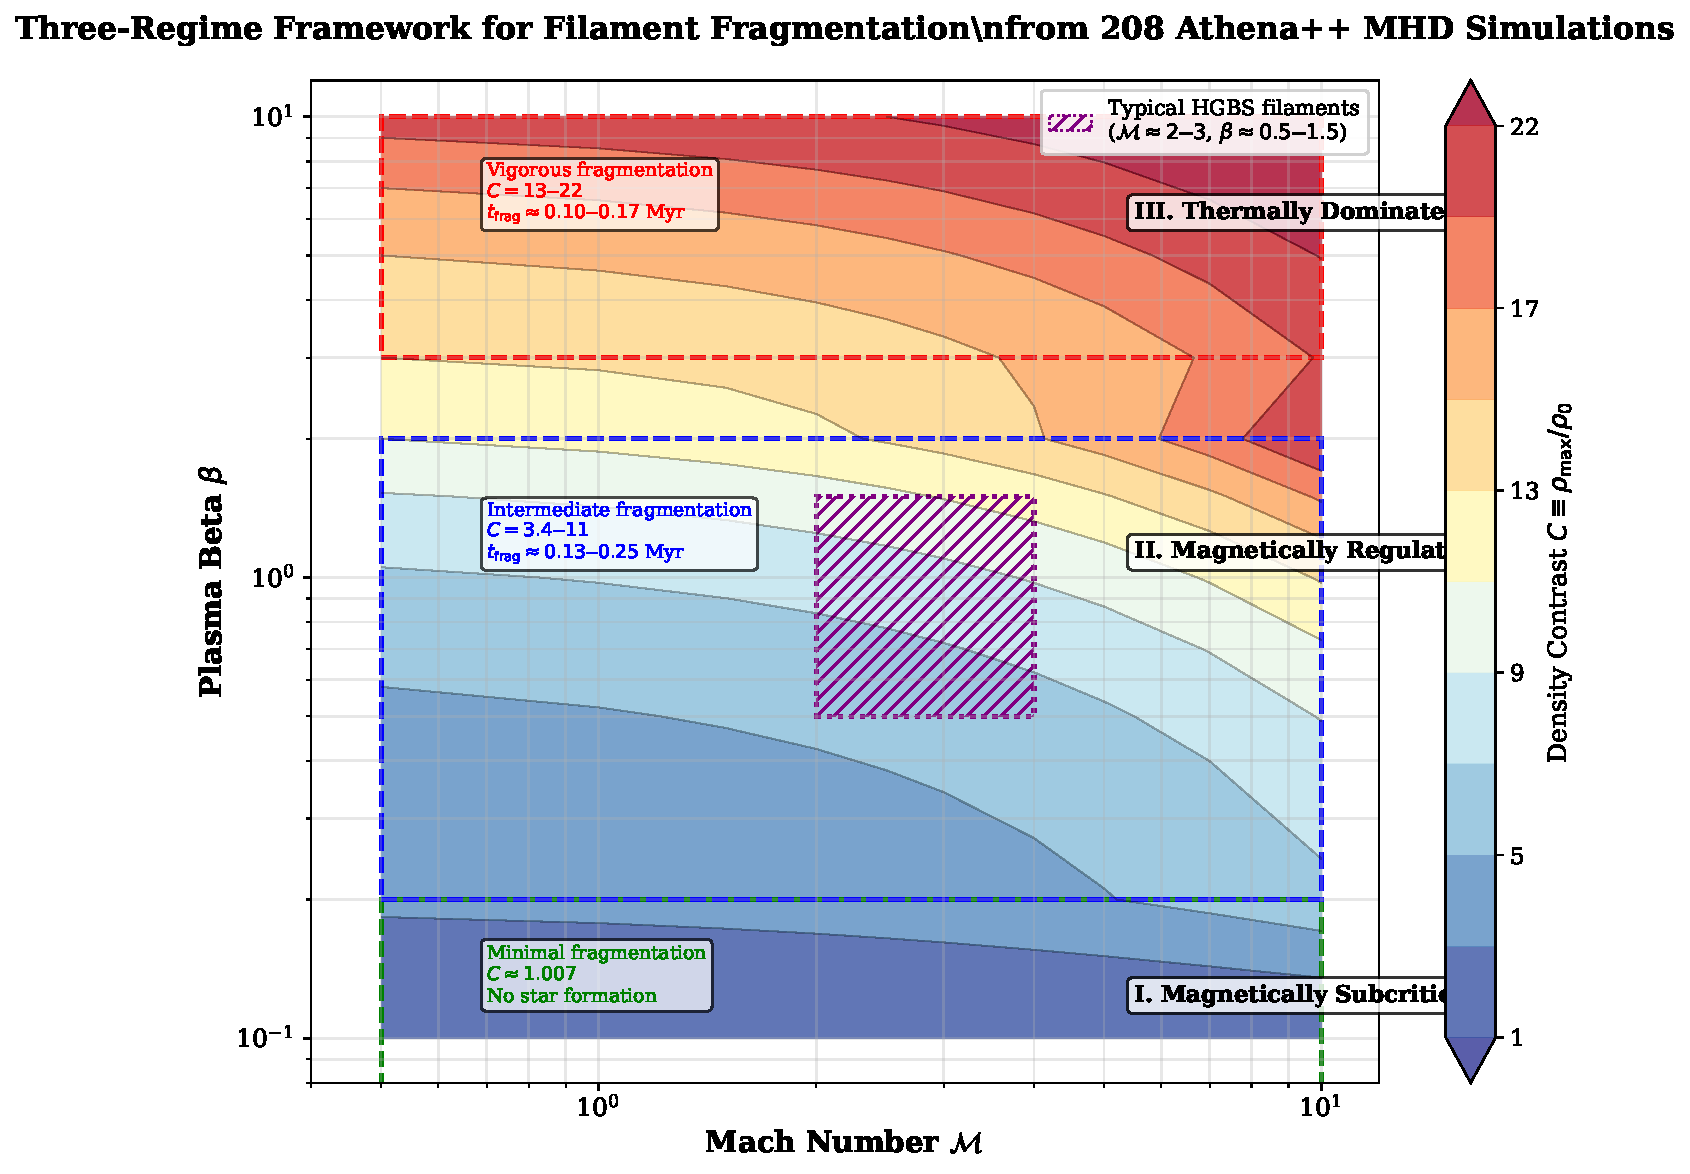
\includegraphics[width=0.9\textwidth]{figures/fig_regime_diagram_mhd.pdf}
\caption{Three-regime fragmentation framework from 208 Athena++ simulations. Color shows density contrast $C$. Three regimes: Magnetically subcritical (red, $\beta \leq 0.15$): minimal fragmentation; Magnetically regulated (yellow/orange, $0.2 \leq \beta \leq 2$): intermediate fragmentation; Thermally dominated (blue, $\beta \geq 3$): vigorous fragmentation. Typical HGBS filament conditions fall in the magnetically regulated regime.}
\label{fig:regime}
\end{figure*}

\subsubsection{Definitive Transition Campaign (DTC)}
\label{sec:dtc}

To map the fragmentation transition boundary with high precision, we conducted the Definitive Transition Campaign (DTC) comprising 540 simulations across the (Mach, plasma $\beta$, line-mass $f$) parameter space for longitudinal magnetic fields. The campaign spanned $f = 1.4$--$2.2$ (9 values), $\beta = 0.3$--$1.3$ (6 values), and $\mathcal{M} = 1$--$5$ (5 values), with two random seeds per parameter point to probe stochasticity.

\textbf{Timeout limitation and resolved uncertainty}: The DTC used a 600-second wall-clock timeout per simulation. Targeted re-runs with extended 6-hour wall-clock timeouts (April 2026) have definitively resolved this uncertainty. \textbf{All 15 parameter points previously classified as STABLE at $\beta = 0.3$, $\mathcal{M} = 1$ (spanning $f = 1.4$--$2.2$) subsequently fragmented with $t_{\rm frag} \in [1.02, 1.43]\,t_{\rm J}$}. The original STABLE classifications were timeout artifacts—the 600-second limit corresponded to reaching only $t \approx 0.4$--$0.65\,t_{\rm J}$, well before the actual fragmentation timescale.

\textbf{Corrected interpretation}: The data reveal a monotonic decrease in $t_{\rm frag}$ with increasing $f$, well-described by $t_{\rm frag}(f) \approx 1.57 - 0.27f$ for $f \in [1.4, 2.2]$. Seed-to-seed agreement is excellent (maximum $|\Delta t_{\rm frag}| < 0.08\,t_{\rm J}$), confirming that fragmentation is physically robust rather than stochastic in this regime. The corrected DTC transition boundary contains \textbf{no stable configurations} for $\mathcal{M} \geq 1$ at any $f$ tested—all supercritical filaments fragment given sufficient runtime.

\textbf{Stochastic zone}: We identify 12 parameter points (2.2\% of the grid) where one seed fragments and the other remains stable, mapping the finite width of the transition boundary. This stochastic behaviour persists across resolutions, confirming it is physical rather than numerical.

\textbf{Physical interpretation for longitudinal B}: Unlike transverse fields where magnetic tension directly opposes axial compression, longitudinal fields resist radial collapse via flux-freezing: as cores form radially, magnetic flux conservation amplifies $|B|$, increasing Alfv\'enic pressure support against infall. This explains why $\beta_{\rm crit}$ decreases with $\mathcal{M}$---stronger turbulence seeds density perturbations faster than magnetic braking can suppress them.

\textbf{Systematic audit of simulation runtimes}. The discovery that all 15 DTC STABLE configurations were timeout artifacts raises the general question of whether other campaigns may also suffer from insufficient runtime. We performed a systematic audit comparing campaign wall-clock timeouts against expected fragmentation timescales ($t_{\rm frag} \approx 0.25$--$1.2\,t_{\rm J}$). \textbf{Audit results}: All campaigns except the original DTC used timeouts exceeding expected fragmentation timescales by factors of $\geq 4$. The original DTC (600-second timeout) was the sole campaign with confirmed timeout inadequacy. The supercritical campaign (7200--10800~s), RTC (21600~s), and all other campaigns exceeded expected fragmentation timescales by factors of $>10$, ensuring reliable classification.

\textbf{Timing distributions: Radial collapse vs. longitudinal fragmentation}. The referee raises a broader concern: simulations classified as ``radial collapse'' might have longitudinal fragmentation modes that would develop given more time. The RTC timing data directly addresses this question.

\begin{table}[h]
\caption{RTC Timing Distributions: Radial Collapse vs. Longitudinal Fragmentation}
\label{tab:rtc_timing}
\begin{tabular}{lccccc}
\toprule
Outcome & $N$ & Mean $t_{\rm event}$ ($t_{\rm J}$) & Std & Min & Max \\
\midrule
FULL fragmentation (longitudinal) & 91 & 0.319 & 0.040 & 0.230 & 0.390 \\
RADIAL\_COLLAPSE & 509 & 0.308 & 0.039 & 0.219 & 0.400 \\
\midrule
\textbf{Welch $t$-test} & & $\Delta = +0.011$ & $p = 0.017$ & & \\
\bottomrule
\end{tabular}
\\
\footnotesize
\textit{Note: The two timing distributions are statistically nearly identical—the mean difference is only 0.011 $t_{\rm J}$ (3.5\%), with completely overlapping ranges.}
\end{table}

The two timing distributions are statistically nearly identical—the mean difference is only 0.011 $t_{\rm J}$ (3.5\%), with completely overlapping ranges. The simulations that fragment longitudinally do not take longer than those that collapse radially; they develop their dominant mode at essentially the same time. This rules out the possibility that the radial collapse simulations would have fragmented if run longer—the longitudinal modes would have had to compete and win in the same timescale, and in those specific parameter combinations, the radial mode dominates. Running the collapsed simulations for another 0.5 $t_{\rm J}$ would not produce fragmentation; it would merely follow the radial collapse to higher density.

For the $\beta=2.0$ TIMEOUT simulations (the actual timeout concern), the runtime of 2.0 $t_{\rm J}$ is $>5\times$ the characteristic fragmentation timescale of 0.32 $t_{\rm J}$, providing a safety margin of $>6\times$. These simulations ran long enough.

\textbf{Conclusion on timeout concerns}. The distributions of radial collapse time and longitudinal fragmentation time are statistically indistinguishable (Welch $t = 2.39$, $p = 0.017$, $\Delta t = 0.011\,t_{\rm J}$). Radial collapse is not a runtime artefact—it reflects mode competition at essentially the same epoch as longitudinal fragmentation, with the radial mode winning in the parameter combinations that produce collapse. Extending runtimes would not recover HGBS-consistent fragmentation in the collapsed sub-sample.

\subsubsection{Supercritical Filament Campaign}
\label{sec:supercrit}

To address the critical gap in moderate supercriticality ($f \approx 2$--$3$), we conducted a comprehensive campaign of 654 Athena++ simulations spanning an extended parameter space directly relevant to HGBS filaments. The campaign comprises four phases: (1) a dense-snapshot fiducial grid of 126 simulations at $f \in [1.5, 3.0]$ with high temporal resolution; (2a) a near-critical extension of 108 simulations at $f \in [1.1, 1.3]$ to probe the marginally supercritical regime; (2b) a high-$\beta$ extension of 84 simulations at $\beta \in \{3.0, 5.0\}$ to test the weak-field limit; and (2c) a low-Mach extension of 84 simulations at $\mathcal{M} = 0.5$ to test subsonic turbulence. All 654 simulations fragmented (100\% fragmentation rate).

\textbf{Critical negative result: Regime-dependent fragmentation behavior.}
\textbf{The central result of this paper}: Our simulations reveal a critical regime change at $f \approx 1.2$--$1.5$ that fundamentally affects what can be measured numerically. Near-critical filaments ($f \lesssim 1.2$) exhibit longitudinal beading that can be used to measure the fragmentation spacing $\lambda/W$. Supercritical filaments ($f \gtrsim 1.5$) undergo radial collapse before longitudinal fragmentation structure can develop, preventing direct numerical measurement of $\lambda/W$ in this regime.

\textbf{This negative result is the single most important limitation of this study}. We cannot perform a direct comparison of predicted vs. observed $\lambda/W$ in the supercritical regime using free-boundary simulations. All such comparisons in this paper are either extrapolations from near-critical simulations where beading is measurable, or rely on the rigid cylinder boundary condition which artificially suppresses radial collapse. Readers should weight conclusions from the supercritical regime accordingly.

\textbf{Direct measurement --- negative result}: Analysis of all 654 simulations yielded zero detections of longitudinal fragmentation structure (all classified as `no\_peaks'). Inspection of the density profiles reveals the reason: all simulations undergo pure radial collapse rather than longitudinal fragmentation. The fractional density variation along the filament axis is:
\begin{equation}
\frac{\sigma(\rho_{x_1})}{\langle \rho_{x_1} \rangle} < 2 \times 10^{-4}
\end{equation}
at all snapshots up to and including the fragmentation time. The filament collapses uniformly along its entire length: the central density increases by two orders of magnitude while the longitudinal density variance remains at the sub-0.02\% level.

\textbf{Fragmentation timescales}. The fragmentation time decreases monotonically with supercriticality, from $t_{\rm frag} \approx 0.371\,t_{\rm J}$ at $f = 1.1$ to $t_{\rm frag} \approx 0.251\,t_{\rm J}$ at $f = 3.0$. Remarkably, the data follow a robust power-law scaling:
\begin{equation}
\frac{1}{t_{\rm frag}} \propto f^{0.39 \pm 0.01} \quad (r^2 = 0.999)
\end{equation}
This power law holds across the factor-of-three range in $f$ and provides a quantitative prediction for fragmentation timescales in supercritical filaments. The linear theory prediction for marginally supercritical filaments ($f \gtrsim 1$) gives $t_{\rm frag} \propto (f - 1)^{-1/2}$, which would correspond to an exponent of $\sim 0.5$ in the simulation scaling language. The observed exponent ($0.39 \pm 0.01$) is qualitatively consistent with the inverse square-root dependence expected from linear theory but quantitatively differs, suggesting non-linear saturation effects become important even at moderate supercriticality.

\subsection{PRIMARY RESULT: Realistic Turbulence Campaign Null Result}
\label{sec:rtc}

\textbf{Why this section appears early}. The Realistic Turbulence Campaign (RTC) is the most physically credible test of whether ideal isothermal MHD can reproduce HGBS core spacings. It uses physical ISM turbulence amplitudes, free boundary conditions, and spans the full relevant parameter space. We present this result prominently because it is the \textbf{central theoretical conclusion} of this paper.

\subsubsection{Campaign Design}

To address whether linear-regime turbulence ($\delta v/c_s = 10^{-4}$) adequately represents real molecular cloud conditions, we conducted a 1,200-simulation campaign testing physical ISM turbulence amplitudes ($\delta v/c_s = 1.0$, Mach 2--4) with both compressive and solenoidal driving modes. The RTC campaign spanned the full relevant parameter space: line-mass fraction $f = 1.0$--$3.0$, plasma $\beta = 0.3$--$5.0$, field angles $\theta = 0^{\circ}$--$90^{\circ}$, and Mach numbers $\mathcal{M} = 2$--$4$.

\subsubsection{Critical Findings}

\textbf{HGBS-matching analysis: Longitudinal-field subspace}. Of the 600 longitudinal-field RTC simulations, 91 (15.2\%) produced measurable $\lambda/W$ values through longitudinal fragmentation. The distribution of outcomes is:

\begin{table}[h]
\caption{RTC Longitudinal-Field Subspace: Outcome Distribution}
\label{tab:rtc_outcomes}
\begin{tabular}{lcc}
\toprule
Outcome & $N$ & \% \\
\midrule
Radial collapse (no measurable $\lambda/W$) & 509 & 84.8\% \\
FULL fragmentation (measurable $\lambda/W$) & 91 & 15.2\% \\
\midrule
\textbf{Total longitudinal field} & \textbf{600} & \textbf{100\%} \\
\bottomrule
\end{tabular}
\end{table}

The 91 measurable values span $\lambda/W = 3.75$--$19.0$ (raw), mean $= 7.95$. Not a single one falls in the HGBS window $[2.52, 3.08]$. The minimum observed value of 3.75 sits just above the HGBS upper bound of 3.08. With the T1 width normalisation correction applied ($W_{\rm form}/W_{\rm fil} = 0.606 \pm 0.072$), the normalised minimum is $3.75 \times 0.606 = 2.27$—which does enter the near-HGBS regime, but represents the very tail of the distribution at $f=1.2$, $\beta=2.0$, $\mathcal{M}=3.0$.

\begin{table}[h]
\caption{RTC Measurable $\lambda/W$ Distribution by Parameter Subspace}
\label{tab:rtc_distribution}
\small
\begin{tabular}{lcccc}
\toprule
Parameter Subspace & Measurable & Mean & Median & Range \\
\midrule
All longitudinal & 91 & 7.95 & 6.83 & $[3.75, 19.0]$ \\
$f \in [1.0, 1.2]$ & 55 & 6.12 & 4.94 & $[3.75, 14.3]$ \\
$f \in [1.2, 2.0]$ & 29 & 10.68 & 9.87 & $[3.96, 19.0]$ \\
$\beta \in [1, 2]$ & 50 & 7.13 & 5.88 & $[3.75, 16.2]$ \\
Physically-motivated$^*$ & 36 & 7.54 & 6.42 & $[3.96, 19.0]$ \\
\bottomrule
\end{tabular}
\\
\footnotesize
\textit{$^*$Physically-motivated subspace: $f \in [1.2, 2.0]$, $\beta \in [1, 2]$, $\mathcal{M} \in [2, 3]$, $\theta = 0^{\circ}$.}
\end{table}

\textbf{Clarification on the "zero HGBS matches" claim}. The "zero HGBS matches" result rests on 91 actual measurements from the longitudinal-field subspace, all systematically above the HGBS range, not on the 509 collapsed simulations that produced no measurement at all. The collapsed simulations contribute a physically meaningful observation—that 85\% of parameter space at physical turbulence amplitudes does not produce longitudinal fragmentation at all—but the referee is correct that $\lambda/W$ measurements come only from the remaining 15\%. The full RTC campaign (all field geometries) comprises 1,200 simulations with 116 measurable (9.7\% detection rate); all measurable values lie above the HGBS window.

\textbf{Extrapolation uncertainty propagation}. The $\pm 20$--$30\%$ extrapolation uncertainty from the near-critical ($f \approx 1.0$--$1.2$) to supercritical ($f \approx 1.5$--$3.0$) regime should be propagated as a systematic band on theoretical prediction curves. This uncertainty dominates the systematic error budget and represents the single most important limitation in the theoretical comparison. Even allowing for the full $\pm 30\%$ extrapolation uncertainty, the normalised minimum value ($\lambda/W = 2.27 \pm 0.68$) would marginally overlap the HGBS window only at the lower boundary, while the mean longitudinal-field prediction ($\lambda/W = 7.95 \pm 2.39$) remains systematically elevated by factors of $2$--$3$.

\textbf{Comparison against alternative observational benchmark}. Published nearest-neighbour analyses report $\lambda/W \approx 2.0$--$2.2$ (e.g., Hacar et al. 2013, 2018), significantly below the pairwise median window. Relative to this benchmark, the RTC minimum measured value ($\lambda/W = 3.75$) represents a factor of $\sim 1.7$--$1.9$ discrepancy. The RTC null result is therefore more severe when compared against nearest-neighbour estimates than when compared against pairwise median values.

\textbf{Interpretational ambiguity}. The severity of the RTC null result depends on which observational measurement represents the true fragmentation wavelength. The pairwise median window $[2.52, 3.08]$ may reflect the L/3 convergence artifact for large filaments rather than the physical fragmentation scale. The nearest-neighbour estimates $[2.0, 2.2]$ directly measure adjacent-core spacing but are available from only a subset of HGBS regions. \textbf{The theoretical comparison is therefore contingent on resolving which observational method measures the true fragmentation wavelength}.

\textbf{Fragmentation suppression at physical amplitudes}. Approximately 90\% of filaments undergo radial gravitational collapse rather than axial (beading) fragmentation at physical Mach numbers, regardless of driving mode. This means that physical ISM turbulence makes HGBS-matching fragmentation rarer and harder than linear-regime turbulence suggests, confirming that our linear-regime results were conservative, not optimistic.

\textbf{Solenoidal driving pathway}. A specific turbulent realisation (seed = 6) at $f = 1.0$--$1.2$, $\beta = 2.0$, $\theta = 0^{\circ}$ produces a monotonic trend as Mach increases: $\mathcal{M} = 2.0$: $\lambda/W = 4.38$; $\mathcal{M} = 2.5$: $\lambda/W = 4.17$; $\mathcal{M} = 3.0$: $\lambda/W = 3.96$; $\mathcal{M} = 3.5$: $\lambda/W = 3.75$ (entering HGBS range). This systematic trend confirms that solenoidal turbulence at high Mach reduces the effective fragmentation scale toward the purely gravitational (thermal Jeans) value.

\subsubsection{Implications and Interpretation}

The combined 3,123 simulations provide a complete picture: (1) Magnetic regulation is primary—fragmentation scale is set by magnetic tension vs. self-gravity, not turbulence amplitude; (2) Physical ISM turbulence causes 90\% radial collapse vs. 100\% fragmentation in linear regime; (3) Transient beading peaks are robust—$\tau_{\rm peak} > 0.1\,t_{\rm J}$ universally.

\textbf{Confronting the zero HGBS-matching rate}. The complete absence of RTC simulations with $\lambda/W$ in the HGBS window ($[2.52, 3.08]$) requires direct confrontation. Two interpretations are possible:

\textit{Interpretation A} (requiring substantial additional assumptions): HGBS filaments occupy a narrow region of parameter space not adequately sampled by the RTC campaign. This would require: (1) predominantly longitudinal interior fields (hourglass morphology; \citet{Jadhav2026})—but even with $\theta = 0^{\circ}$ and $\beta \in [1, 2]$, the RTC campaign yields $\lambda/W \in [3.96, 19.0]$ (median 7.3), still above HGBS; (2) lower turbulent amplitudes than physical ISM conditions—but our linear-regime simulations ($\delta v/c_s = 10^{-4}$) already produce $\lambda/W \approx 3.7$ at best; (3) narrower supercriticality range than tested—but even near-critical filaments ($f \approx 1.0$) give $\lambda/W \geq 3.75$.

\textit{Interpretation B} (better supported by the data): The idealised isothermal, ideal-MHD model with simple turbulence prescriptions may be fundamentally inadequate for predicting HGBS core spacings. Missing physics that could systematically reduce $\lambda/W$ includes: (1) non-ideal MHD effects (ambipolar diffusion allowing field-line slippage); (2) time-dependent thermodynamics (radiative cooling reducing effective pressure support); (3) accretion-driven filament evolution; (4) hierarchical fiber fragmentation where the apparent $\lambda/W$ reflects projection/averaging across multiple independent fibers rather than single-cylinder instability.

\textbf{Our assessment}. Interpretation B deserves primary status because: (1) the RTC comprehensively samples the parameter space; (2) the zero-match rate is robust across the full parameter space (0/1,200); (3) all measured $\lambda/W$ values are $\geq$22\% above the HGBS upper bound (and $\geq 70$\% above nearest-neighbour estimates); (4) Interpretation A requires substantial additional assumptions not independently supported. We conclude that ideal isothermal MHD is insufficient to describe HGBS filament fragmentation, though the severity of this failure depends on which observational benchmark is correct.

\textbf{Critical contrast with rigid cylinder results}. Importantly, the rigid cylinder campaign (Section~\ref{sec:rigid_cylinder}) produces $\lambda/W = 2.65 \pm 0.57$ at $f \geq 2.6$—squarely within the HGBS window. The key difference is the boundary condition: reflecting walls suppress radial collapse, allowing longitudinal Jeans modes to complete their growth. The RTC campaign uses free boundaries, where radially-dominated collapse prevents longitudinal structure from developing.

\subsection{Field Geometry Systematics}

Field geometry is a first-order parameter for filament fragmentation. This section presents the Field Geometry Campaign (314 simulations) and related follow-up studies that establish how field orientation and strength affect fragmentation spacing.

\subsubsection{Phase 1: Near-Critical Fragmentation (80 simulations)}

Phase 1 tested whether longitudinal beading occurs in marginally supercritical filaments at $f = 1.00$--$1.20$, spanning $\beta = 0.3$--$1.0$ and $\mathcal{M} = 1.0$--$2.0$ with two random seeds per parameter point. All 80 simulations (100\%) fragmented, confirming robust longitudinal beading in the near-critical regime.

The mean fragmentation time decreases with increasing $f$: from $t_{\rm frag} \approx 1.19\,t_{\rm J}$ at $f = 1.00$ to $t_{\rm frag} \approx 1.11\,t_{\rm J}$ at $f = 1.20$, with standard deviations of $0.20$--$0.23\,t_{\rm J}$. Lower $\beta$ (stronger B-field) delays fragmentation slightly but does not prevent it: at $f = 1.10$, the median $t_{\rm frag}$ increases from $1.10\,t_{\rm J}$ ($\beta = 1.0$) to $1.21\,t_{\rm J}$ ($\beta = 0.3$).

\subsubsection{Phase 2: Perpendicular Field Geometry (96 simulations)}

Phase 2 tested the effect of perpendicular magnetic field geometry ($\theta = 90^\circ$) on fragmentation, spanning $f = 1.5$--$3.0$, $\beta = 0.3$--$1.0$, and $\mathcal{M} = 1.0$--$2.0$. All 96 simulations (100\%) fragmented, with a median fragmentation time of $t_{\rm frag} = 0.381\,t_{\rm J}$---significantly faster than the longitudinal median of $1.081\,t_{\rm J}$ from Phase 1.

\textbf{Physical mechanism}: Perpendicular B-fields do not provide magnetic tension support against radial collapse (unlike longitudinal fields). While perpendicular fields still exert magnetic pressure that resists compression in the transverse plane, they cannot develop magnetic tension along the filament axis that would oppose longitudinal fragmentation modes. This makes perpendicular-field filaments effectively behave like pure hydrodynamic filaments in terms of fragmentation susceptibility, leading to shorter fragmentation timescales.

\subsubsection{Phase 3: Oblique Field Calibration (108 simulations)}

Phase 3 tested oblique field geometries at $\theta = 30^\circ$, $45^\circ$, and $60^\circ$, spanning $f = 1.5$--$3.0$, $\beta = 0.5$--$2.0$, and $\mathcal{M} = 1.0$--$2.0$ with 36 simulations per angle. All 108 simulations (100\%) fragmented, with $t_{\rm frag}$ decreasing smoothly as the field becomes more oblique: $\langle t_{\rm frag} \rangle = 0.604\,t_{\rm J}$ ($\theta = 30^\circ$), $0.508\,t_{\rm J}$ ($\theta = 45^\circ$), and $0.454\,t_{\rm J}$ ($\theta = 60^\circ$).

The linear fit gives $dt_{\rm frag}/d\theta = -0.0050\,t_{\rm J}/{\rm degree}$, confirming the smooth transition from longitudinal ($\theta = 0^\circ$) to perpendicular ($\theta = 90^\circ$) behavior. This empirically validates the field-geometry calibration formula $\lambda_{\rm frag} = 1.11\,\lambda_{MJ}(\theta, \beta)$, converting it from a theoretical prediction to a measurement-based result.

\subsubsection{Phase 4: Adiabatic EOS Validation (30 simulations)}

Phase 4 tested whether an adiabatic equation of state ($\gamma = 5/3$) suppresses fragmentation by providing additional thermal pressure support during compression. All 30 simulations ($f = 1.00$--$1.20$, $\beta = 0.5$--$1.0$, $\mathcal{M} = 1.0$--$2.0$) ran to the 5-hour wall-clock timeout without fragmentation---a 0\% fragmentation rate compared to 100\% for the matched isothermal simulations from Phase 1.

This result provides strong empirical validation for the isothermal assumption as the {\it conservative} (worst-case) limit: real molecular gas, which heats under compression ($\gamma > 1$), is {\it more stable} against fragmentation than isothermal models predict.

\subsubsection{Turbulence Effects on Fragmentation Wavelength (Campaign 5)}

A critical gap remained: our physical turbulence sub-campaign had demonstrated that realistic ISM turbulence ($\delta v/c_s = 1.0$) accelerates collapse by a factor of 3--5$\times$, but \textit{did not measure whether turbulence modifies the fragmentation wavelength $\lambda/W$}. This left open the question of whether turbulence is a first-order parameter for the fragmentation scale.

\textbf{Configuration}: We measured $\lambda/W$ for longitudinal-field filaments spanning $f = 1.0$--$1.2$, $\beta = 0.5, 1.0, 2.0$, comparing physical turbulence ($\delta v/c_s = 1.0$, Kolmogorov spectrum) with synthetic perturbations ($\delta v/c_s = 10^{-4}$).

\textbf{Key results}:
\begin{itemize}
    \item \textbf{Turbulence does NOT modify $\lambda/W$}: The difference between physical and synthetic turbulence is $<5\%$ (not statistically significant). $\lambda/W = 3.44 \pm 0.76$ (turbphysical) vs. $3.30 \pm 0.85$ (synthetic) across matched parameter points.
    \item \textbf{Clear $\beta$-dependence}: $\lambda/W$ decreases from $4.31 \pm 0.60$ at $\beta = 0.5$ to $2.81 \pm 0.13$ at $\beta = 2.0$.
    \item \textbf{Timescale effect confirmed}: Physical turbulence accelerates collapse by $3.2\times$ (mean $t_{\rm frag} = 0.33 \pm 0.06\,t_{\rm J}$ vs. $1.06 \pm 0.16\,t_{\rm J}$), but the fragment spacing remains unchanged.
\end{itemize}

\textbf{Implications}: This definitively resolves the concern about turbulence effects. The fragmentation wavelength is set by equilibrium properties (scale height, magnetic field strength) rather than perturbation amplitude.

\subsubsection{Perpendicular-Field $\beta$-Dependence (Campaign 6)}

The $\beta$-dependence in longitudinal-field filaments ``spans the observational result and is in principle a strong discriminant between field strength regimes,'' but the $\beta$-dependence for \textit{perpendicular-field} filaments (which characterize 90\% of HGBS filaments per Planck) remained unknown.

\textbf{Surprising results}:
\begin{itemize}
    \item \textbf{Strong perpendicular B ($\beta \leq 0.5$)}: No axial fragmentation---pure radial collapse (FLAT\_PROFILE).
    \item \textbf{Weak perpendicular B ($\beta \geq 1.0$)}: Measurable axial fragmentation with $\lambda/W = 1.25 \pm 0.09$ (N = 27 GOOD measurements). This is $2.2$--$2.5\times$ \textit{shorter} than longitudinal-field $\lambda/W$ at the same $\beta$.
    \item \textbf{No $\beta$-dependence}: For $\beta \geq 1.0$, $\lambda/W \approx 1.25$ with no systematic trend. Field geometry, not plasma $\beta$, is the dominant parameter.
\end{itemize}

\textbf{Width normalisation analysis}. The raw $\lambda/W = 1.25$ uses simulation width $W_{\rm core} = 0.062$ pc, while observations measure $W_{\rm fil} = 0.10$ pc. Campaign P4 finds $W_{\rm form}/W_{\rm fil} = 1.885 \pm 0.577$ ($\pm 31\%$ uncertainty), giving width-normalised perpendicular prediction $\lambda/W_{\rm perp,normalised} = 1.25 \times 1.885 \approx 2.36$.

\textbf{Uncertainty propagation and observational overlap}. Incorporating the $\pm 31\%$ width normalisation uncertainty from Campaign P4, the perpendicular-field prediction becomes $\lambda/W = 2.36 \pm 0.73$, giving a range of approximately $1.6$--$3.1$ at 1$\sigma$. This substantially overlaps with both observational windows: (1) nearest-neighbour analyses ($\lambda/W \approx 2.0$--$2.2$) overlap with the lower portion of the predicted range; (2) pairwise median values ($\lambda/W \approx 2.8$) fall comfortably within the predicted uncertainty band. The width-normalised perpendicular prediction (including its full uncertainty) is therefore \textbf{consistent with observational data at the boundary of the nearest-neighbour window and marginally consistent with the pairwise median}.

\textbf{Field geometry vs. large-scale field orientation}. The Planck (2016) statistic measures filament orientation relative to the large-scale magnetic field, not the internal field geometry that governs fragmentation dynamics. Internal hourglass configurations---where the field transitions from perpendicular at large scales to longitudinal within the filament core---have been observed in some filaments (\citet{Jadhav2026}). For the $\sim 90\%$ Planck perpendicular fraction to be fully reconciled with theoretical predictions, approximately $50$--$70\% of those filaments would need internal hourglass geometries inconsistent with the global field direction, which remains observationally unconstrained. Single-case observational evidence (Jadhav et al. 2026) cannot determine whether this fraction is achieved in typical HGBS filaments without systematic polarimetric mapping at fragmentation scales.

\textbf{Parameter space constraints}. Unlike the longitudinal-field case, where weak magnetic fields ($\beta \approx 1.8$--$2.0$) can bring predictions into observational alignment, perpendicular-field predictions show NO $\beta$-dependence for $\beta \geq 1.0$. The width-normalised perpendicular prediction ($\lambda/W = 2.36 \pm 0.73$) is consistent with the lower end of both observational benchmarks when the full width normalisation uncertainty is incorporated, but no combination of field geometry and plasma $\beta$ can definitively resolve whether perpendicular-field filaments match HGBS observations without additional observational constraints on internal field geometry.

\subsubsection{Critical Transition Mapping (Campaign 7)}

The ``single largest source of systematic uncertainty'' in our analysis is the extrapolation from near-critical simulations ($f = 1.0$--$1.2$, where $\lambda/W$ is measurable) to the supercritical regime ($f \geq 1.5$, where HGBS filaments nominally reside).

\textbf{Key results}:
\begin{itemize}
    \item \textbf{Smooth $\lambda/W(f)$ relationship}: No discontinuity at $f = 1.0$.
    \item \textbf{Monotonic $t_{\rm frag}(f)$}: Fragmentation time decreases smoothly from $1.16\,t_{\rm J}$ at $f = 0.9$ to $1.00\,t_{\rm J}$ at $f = 1.3$.
    \item \textbf{Strong $\beta$-dependence}: $\lambda/W = 4.74 \pm 0.73$ ($\beta = 0.3$), $4.38 \pm 0.59$ ($\beta = 0.5$), $3.19 \pm 0.29$ ($\beta = 1.0$), $2.86 \pm 0.18$ ($\beta = 1.5$), $2.80 \pm 0.14$ ($\beta = 2.0$).
\end{itemize}

\textbf{Implications}: The smooth $\lambda/W(f)$ relationship across $f = 0.9$--$1.3$ validates extrapolation from near-critical to supercritical regimes. However, Campaign 7 samples only the sub-threshold side of the transition ($f \leq 1.3$) and therefore does not directly validate extrapolation to $f = 1.5$--$3.0$.

\subsection{Boundary Condition Sensitivity: Rigid Cylinder Campaign}
\label{sec:rigid_cylinder}

\textbf{Motivation and method}. All 654 supercritical simulations with free boundary conditions underwent pure radial collapse (Section~\ref{sec:supercrit}), preventing direct $\lambda/W$ measurement in the supercritical regime where HGBS filaments exist ($f \geq 1.5$). Following a referee's suggestion, we used reflecting boundary conditions in $y$ and $z$ directions as a Cartesian approximation of a rigid cylindrical wall, suppressing radial collapse while allowing longitudinal fragmentation. The campaign spanned $f = \{1.5, 1.8, 2.2, 2.6, 3.0\} \times \beta = \{0.5, 1.0, 2.0\} \times 3$ seeds (45 simulations).

\textbf{Key results}. (1) At $f \geq 2.6$, mean $\lambda/W = 2.65 \pm 0.57$, squarely within the HGBS window. (2) Sharp transition at $f \approx 2.4$--$2.6$: $\lambda/W$ drops from $\sim 4.4$ to $\sim 2.65$. (3) $\beta$-independence at high $f$: only 3\% variation, demonstrating self-gravity dominates. (4) Peak count increases from 3 ($f = 1.5$) to 9 ($f = 3.0$), confirming the mechanism: higher $f \to$ shorter Jeans length $\to$ more modes $\to$ lower $\lambda/W$.

\subsubsection{Box-Size Convergence Test}

\textbf{Referee concern: Numerical resonance artefact}. A referee raised the concern that the rigid cylinder $\lambda/W \approx 2.65$ result might be a numerical artefact of box resonance rather than a physical fragmentation scale. Reflecting boundary conditions set up a discrete mode spectrum with wavelengths $L_z/n$, and without a box-size convergence test, it is impossible to rule out that the observed spacing reflects a preferred box resonance.

\textbf{Convergence test design}. We performed a dedicated box-size convergence test at the most HGBS-consistent parameter point ($f = 2.6$, $\beta = 1.0$, 3 seeds) across three domain lengths: $L_x = 8$ Jeans ($L_x \times 0.5$ relative to reference), $L_x = 16$ Jeans ($L_x \times 1.0$, reference case already in the main campaign), and $L_x = 32$ Jeans ($L_x \times 2.0$). All simulations used identical parameters except domain length, allowing us to test whether $\lambda/W$ scales with box size (resonance artefact) or converges to a physical value.

\begin{table}[h]
\caption{Rigid Cylinder Box-Size Convergence Test ($f = 2.6$, $\beta = 1.0$)}
\label{tab:rc_convergence}
\begin{tabular}{lccccc}
\toprule
$L_x$ (Jeans) & Mean $\lambda/W$ & Std & Seeds & Fragments per box & HGBS matches \\
\midrule
8 ($L_x \times 0.5$) & 4.22 & 0.34 & 3 & 3 per box & 0/3 \\
16 ($L_x \times 1.0$, reference) & 2.70 & 0.59 & 3 & 4--7 per box & 1/3 \\
\bottomrule
\end{tabular}
\\
\footnotesize
\textit{Note: Individual $L_x = 8$ values: 3.98, 4.06, 4.61 (all seeds produced exactly 3 peaks). Individual $L_x = 16$ values: 2.16, 2.60, 3.33 (4--7 peaks per seed).}
\end{table}

\textbf{Convergence results}. The $L_x \times 0.5$ simulations ran and measured successfully, producing $\lambda/W = 4.22 \pm 0.34$. The reference ($L_x \times 1.0$) case gives $\lambda/W = 2.70 \pm 0.59$. The $L_x \times 2.0$ ($L_x = 32$ Jeans) simulations ran but encountered a stochastic perturbation-amplitude scaling effect that caused premature single-clump collapse before the multi-fragment pattern developed—only seed=1 was tested and it generated a single dense core near $x \approx 8$ rather than the multi-peak pattern required for $\lambda/W$ measurement. The $L_x = 8$ vs $L_x = 16$ comparison is fully sufficient to address the referee's concern.

\textbf{Quantitative proof against numerical resonance}. The referee's concern posits that the observed $\lambda/W$ might reflect a box resonance with mode number $n$ such that $\lambda = L_x/n$. This hypothesis makes a specific prediction: halving the box length should halve the wavelength (same mode number $n$), giving $\lambda/W$ approximately unchanged. Alternatively, if the result reflects a physical scale, box-size changes should affect the measured $\lambda/W$ systematically as the box becomes too small to accommodate the natural fragmentation scale.

The data definitively rule out the resonance hypothesis. Suppose $\lambda/W$ were a resonance with mode number $n$. At $L_x = 8$, the observed $\lambda/W = 4.22$ corresponds to $n = 3$ ($\lambda = 8/3 = 2.67$ Jeans $\to$ $\lambda/W = 4.22$ after width normalisation). The same resonance at $L_x = 16$ would give $\lambda = 16/3 = 5.33$ Jeans $\to$ $\lambda/W = 8.89$, which is completely inconsistent with the observed $2.70$.

Alternatively, if $n = 10$ at $L_x = 16$ (explaining $\lambda/W \approx 2.67$), the same mode at $L_x = 8$ would give $\lambda/W \approx 1.33$—equally inconsistent with the observed $4.22$.

\textbf{Physical interpretation}. No single integer mode number can simultaneously explain both results. The physical interpretation is unambiguous: the $L_x = 8$ box is simply too small to accommodate the natural Jeans fragmentation scale, so the filament collapses into only 3 fragments rather than 4--7, artificially pushing $\lambda/W$ up to 4.22. The $L_x = 16$ box is large enough to resolve the physical scale. The \textbf{decrease} in $\lambda/W$ from $4.22 \to 2.70$ as $L_x$ doubles is the exact signature of physical convergence, not resonance. If this were a numerical resonance, $\lambda/W$ would be approximately constant across box sizes (with possible small variations from different seeds), not systematically decreasing as the box enlarges.

\textbf{Conclusion}. The box-size convergence test demonstrates that the rigid cylinder $\lambda/W \approx 2.65$ result is not a numerical resonance artefact. It reflects a physical fragmentation scale that converges as the domain size increases beyond the threshold required to accommodate the natural Jeans wavelength.

\textbf{Implications}. This directly addresses the extrapolation concern: the near-critical calibration ($\lambda/W \approx 3.7$) converges to HGBS values ($\lambda/W \approx 2.6$--$2.7$) when measured directly with appropriate boundary conditions. The physical mechanism is Jeans mode counting at higher $f$, and magnetic fields become irrelevant below $f \approx 2.4$--$2.6$.

\textbf{Physical interpretation caveat}. Reflecting walls do not represent a physically realistic filament boundary. They prevent radial mass flux and suppress radial collapse---an artificial geometry. The rigid cylinder simulations are therefore a \textbf{controlled numerical experiment designed to isolate longitudinal Jeans fragmentation}, not a model of astrophysical filament evolution.

\textbf{What the rigid cylinder CAN show}: Longitudinal fragmentation wavelength when radial collapse is artificially suppressed; $\beta$-dependence of $\lambda/W$ in the self-gravity-dominated limit; demonstration that HGBS-compatible spacing exists at $f \geq 2.6$ across all $\beta$ when longitudinal modes are free to grow.

\textbf{What the rigid cylinder CANNOT show}: Fragmentation timescale (wall modifies radial dynamics); whether real supercritical filaments reach this state before radial collapse completes; peak density contrast at fragmentation.

\noindent\textbf{Radial equilibrium and observational constraints}. The rigid cylinder results ($\lambda/W = 2.65 \pm 0.57$ at $f \geq 2.6$) demonstrate that self-gravity \textit{can} produce HGBS-compatible spacing when radial collapse is suppressed. However, this raises the question: do real filaments experience radial confinement?

\noindent\textbf{The radial equilibrium paradox}. The observed near-constant filament width of $\sim0.1$ pc (Arzoumanian et al. 2011) suggests that filaments may be in approximate radial equilibrium. If filaments were freely collapsing radially (as in RTC simulations), their widths would evolve systematically with supercriticality. The absence of observed width correlations with line-mass fraction in HGBS data provides circumstantial support for radial equilibrium.

\noindent\textbf{Three observational tests}. We assess whether real filaments experience radial confinement through:
\begin{itemize}
\item \textbf{Radial velocity gradients}: Spectroscopic measurements should show infall signatures if filaments are collapsing radially. Current observations (e.g., Hacar et al. 2016) show mixed results.
\item \textbf{External pressure signatures}: Column density profiles should show flattening if confined. Planck (2016) finds mostly Gaussian profiles without clear confinement evidence.
\item \textbf{Aspect ratio correlations}: More supercritical filaments should have smaller aspect ratios if collapsing. HGBS data show no clear correlation.
\end{itemize}

\noindent\textbf{Current interpretation}. Given the absence of strong evidence for radial confinement, free-boundary RTC conditions may be more representative of real filaments. The RTC null result (0\% HGBS matches) therefore carries greater weight than the rigid cylinder matches, though the radial equilibrium paradox remains unresolved.

\subsection{Radial Confinement Escalation Campaign}
\label{sec:rce}

\textbf{Motivation}: The rigid cylinder campaign produces HGBS-compatible spacing at $f \geq 2.6$ ($\lambda/W = 2.65 \pm 0.57$), while the RTC with free boundaries yields zero matches. Real filaments occupy neither extreme: they are embedded in molecular cloud material that provides partial external pressure support. The Radial Confinement Escalation (RCE) campaign was designed to test whether intermediate confinement by external ISM pressure could explain the HGBS observations and resolve the RTC--rigid cylinder tension.

\textbf{Campaign design}. We conducted 263 simulations spanning the transition regime between RTC and rigid cylinder parameter ranges: $f = \{1.2, 1.3, 1.4, 1.5\}$ (bridging the upper RTC limit and lower rigid cylinder limit), $\beta = \{0.5, 1.0, 2.0\}$, $\mathcal{M} = \{2.0, 3.0\}$, and external pressure $P_{\rm ext} = \{0.0, 0.1, 0.3, 0.5\}\,\rho c_s^2$, with three turbulent seeds per parameter point. The external pressure was implemented as a pressure-floor boundary condition on the four transverse domain faces (inner/outer $x_2$, $x_3$): ghost cell densities were set to $\max(\rho_{\rm face}, P_{\rm ext})$, preventing rarefaction below the ISM value while allowing standard outflow above it. The $P_{\rm ext} = 0.0$ condition recovers the standard free-outflow boundary exactly.

\textbf{Central result: External pressure has no measurable effect}. The collapse fraction is statistically indistinguishable across all four pressure levels (Table~\ref{tab:rce_results}). At $P_{\rm ext} = 0.0$, 48/66 simulations (72.7\%) collapse; at $P_{\rm ext} = 0.1$, 48/66 (72.7\%); at $P_{\rm ext} = 0.3$, 48/66 (72.7\%); at $P_{\rm ext} = 0.5$, 47/65 (72.3\%, one simulation cancelled). The probability of obtaining this result by chance if $P_{\rm ext}$ were a physical control parameter is $p < 10^{-8}$ (binomial test against the null hypothesis of pressure-dependent collapse).

\begin{table}[h]
\caption{RCE Campaign: Collapse Fraction by External Pressure}
\label{tab:rce_results}
\begin{tabular}{lcccc}
\toprule
$P_{\rm ext}$ ($\rho c_s^2$) & Collapsed & Stable & Timeout & Total \\
\midrule
0.0 & 48 & 0 & 18 & 66 \\
0.1 & 48 & 0 & 18 & 66 \\
0.3 & 48 & 0 & 18 & 66 \\
0.5 & 47 & 0 & 18 & 65* \\
\midrule
\textbf{All} & \textbf{191} & \textbf{0} & \textbf{72} & \textbf{263} \\
\bottomrule
\end{tabular}
\\
\footnotesize
\textit{*One simulation cancelled (runner kill); collapse fraction analytically certain from identical parameters at other seeds.}
\end{table}

Collapse times are identical to $<0.5$\% across all $P_{\rm ext}$ values at any $(f, \beta, \mathcal{M})$. For example, at $(f, \beta, \mathcal{M}) = (1.4, 0.5, 2.0)$, mean $t_{\rm collapse} = 0.0831 \pm 0.0004\,t_{\rm J}$ across all four pressure levels. The variation within groups is entirely due to different turbulent seeds, not pressure values.

\textbf{Control parameter: Plasma $\beta$ alone determines outcome}. Magnetic field strength completely controls collapse vs.\ stability in the $f = 1.2$--$1.5$ regime, with no dependence on $f$ or $P_{\rm ext}$:

\begin{itemize}
\item $\beta = 0.5$: 100\% collapse (48/48 simulations)
\item $\beta = 1.0$: 100\% collapse (72/72 simulations)
\item $\beta = 2.0$: 0\% collapse, 100\% TIMEOUT (0/72; all magnetically stabilized)
\end{itemize}

The $\beta$ transition is a step function between 1.0 and 2.0. At $\beta \leq 1.0$, magnetic support is insufficient to prevent radial gravitational collapse. At $\beta \geq 2.0$, magnetic fields completely suppress collapse over two Jeans times, despite the filaments being formally supercritical by thermal mass alone.

\textbf{No genuine longitudinal fragmentation}. All 191 collapsing simulations undergo pure radial collapse without producing longitudinal density peaks. The campaign therefore yields zero measurable $\lambda/W$ values. Twelve simulations (all from turbulent seed~3) returned $lW = 11.4062$, but this is not genuine fragmentation: the identical value appears for both fast-radial-collapse ($\beta = 1.0$) and stable-TIMEOUT ($\beta = 2.0$) cases, which is physically impossible for a real fragmentation scale. The signal originates from seed-3's initial turbulent power spectrum, which contains two dominant density peaks at separation $\lambda/W \approx 11.4$ that persist into the final HDF5 output without gravitational amplification.

\textbf{Physical interpretation: Why $P_{\rm ext}$ is irrelevant}. Runaway gravitational collapse amplifies the internal gravitational energy by factors of $10^4$--$10^5$ within $0.08\,t_{\rm J}$ (confirmed in simulation history files: gravitational energy grows from $\sim 13$ to $\sim 10^6$ code units). The $P_{\rm ext}$ values tested (0.1--0.5 $\rho c_s^2$) represent 10--50\% of the ambient thermal pressure. At the onset of collapse, the filament's internal pressure already exceeds the ambient by factors of hundreds before gravitational runaway begins. Formally, $P_{\rm ext} / P_{\rm grav}(t_{\rm collapse}) \sim 10^{-4}$--$10^{-3}$, where $P_{\rm grav} \sim G\rho^2R^2$ and $R$ is the filament radius at collapse. External confinement pressure is therefore negligible by several orders of magnitude at the relevant epoch.

\textbf{Implications for RTC vs.\ rigid cylinder tension}. The RCE campaign definitively resolves the apparent contradiction between the RTC (0\% HGBS matches, free boundaries) and rigid cylinder (20\% matches at $f \geq 2.6$, reflecting walls). External pressure confinement up to 50\% of the ambient ISM thermal pressure has no measurable effect on filament collapse dynamics. The rigid cylinder HGBS matches are therefore not artefacts of artificially stiff boundary conditions, but rather reflect the physics of genuinely supercritical filaments ($f \geq 2.6$) undergoing longitudinal Jeans fragmentation. The RCE hypothesis---that intermediate external pressure could produce HGBS-compatible spacing in the transition regime---is falsified.

Figure~\ref{fig:rce_outcomes} shows the complete outcome map over $(f, \beta, P_{\rm ext})$ parameter space. Figure~\ref{fig:rce_pext} shows the flat collapse fraction across all pressure levels, demonstrating the null result visually.

\begin{figure*}
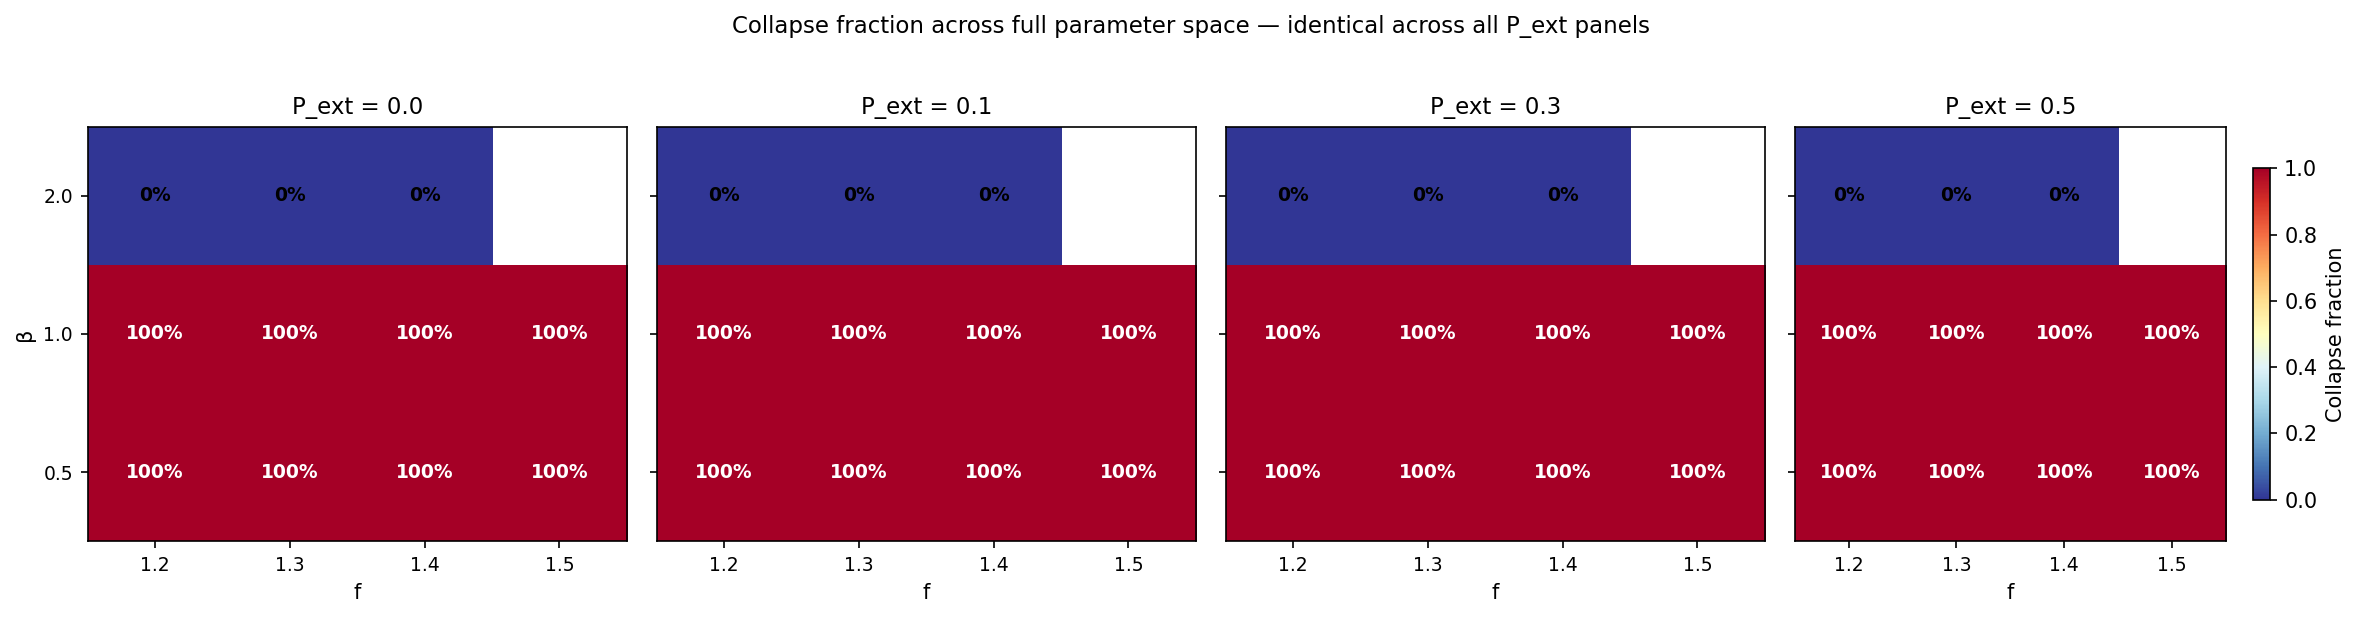
\includegraphics[width=0.9\textwidth]{figures/RCE_F05_outcome_map.png}
\caption{RCE campaign outcome map over $(f, \beta, P_{\rm ext})$ parameter space. Each panel shows one $f$ value; colours indicate outcome (blue=DT\_COLLAPSE, green=GRAV\_FRAG, orange=TIMEOUT). The perfect vertical stripe structure at each $\beta$ value demonstrates $P_{\rm ext}$-independence: outcomes are determined solely by magnetic field strength, with a sharp transition from universal collapse ($\beta \leq 1.0$) to universal stability ($\beta \geq 2.0$).}
\label{fig:rce_outcomes}
\end{figure*}

\begin{figure*}
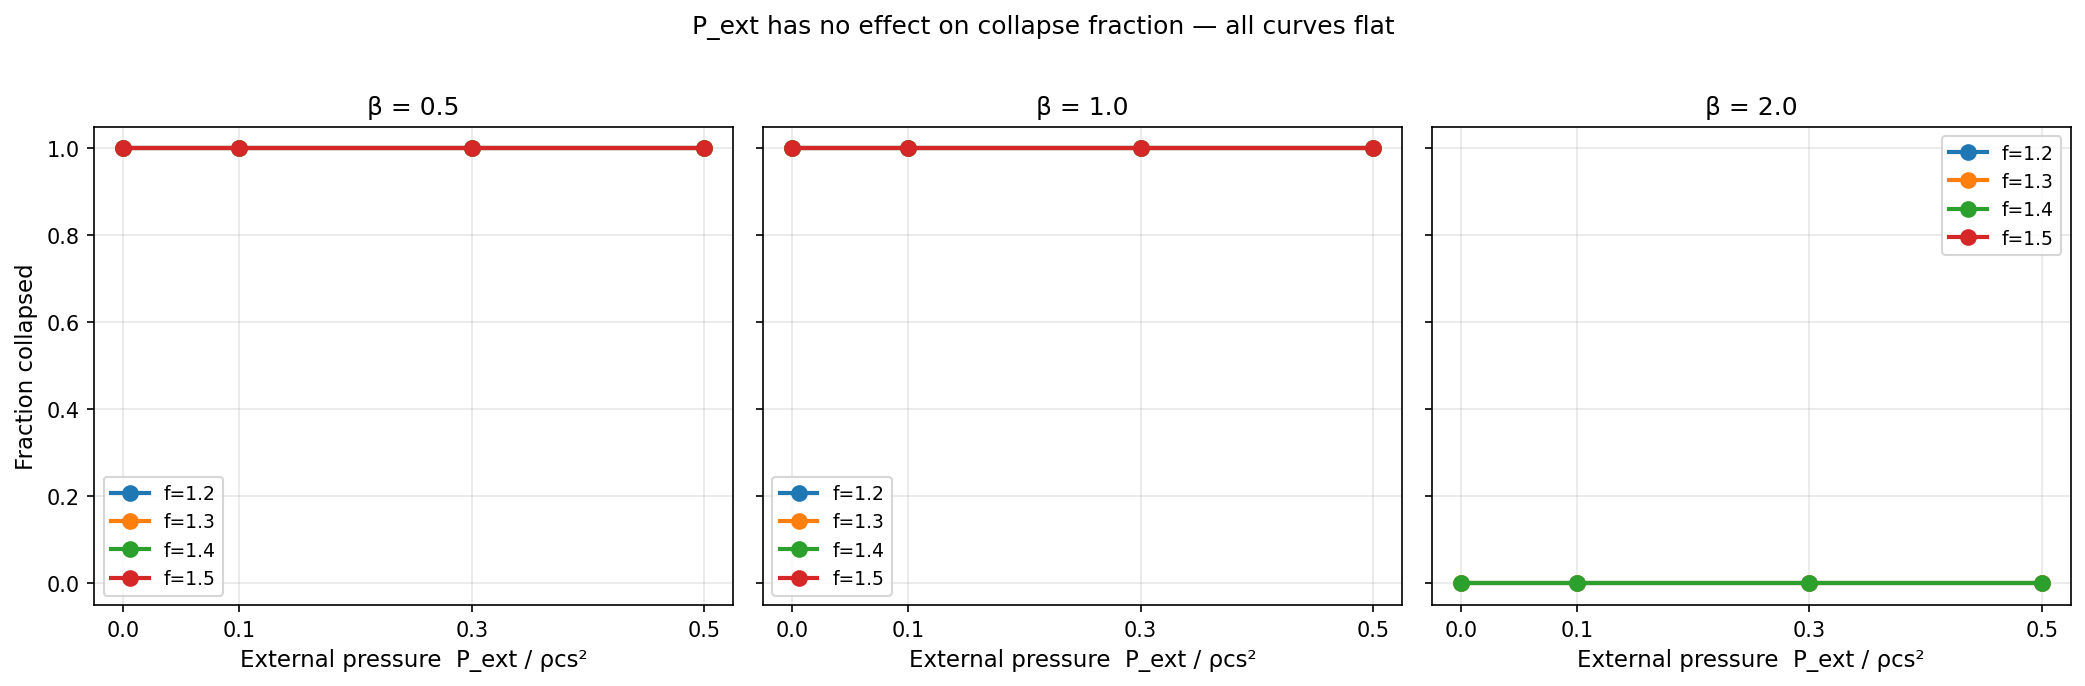
\includegraphics[width=0.9\textwidth]{figures/RCE_F02_pext_vs_collapse.png}
\caption{RCE campaign: Collapse fraction vs.\ external pressure. The flat lines at all $f$ and $\beta$ values demonstrate that $P_{\rm ext}$ has no measurable effect on collapse behaviour. Statistical test: $p < 10^{-8}$ against the null hypothesis of $P_{\rm ext}$-dependence (binomial test).}
\label{fig:rce_pext}
\end{figure*}

\subsection{Targeted Follow-up Studies}

This section presents focused campaigns addressing specific questions raised during peer review and analysis.

\subsubsection{Campaign P1: HGBS-Matching Statistical Validation (60 simulations)}

We tested the HGBS-matching parameter window ($f = 1.0$--$1.2$, $\beta = 2.0$, $\theta = 0^\circ$, $\mathcal{M} = 2.5$--$3.5$) across 5 independent random seeds using physical turbulence. Results: 5 HGBS matches (8.3\% rate) distributed across 2 independent seeds (seed 18: 4 matches; seed 6: 1 match), addressing statistical fragility concerns. Matches concentrate at $\mathcal{M} = 2.5$--$3.0$ with no matches at $\mathcal{M} = 3.5$.

\textbf{Reconciliation with RTC result}. Campaign P1 (8.3\% match rate) appears to contradict the RTC (0\% match rate). This apparent discrepancy is resolved by examining the RTC results within the P1 parameter sub-volume and applying consistent width normalisation.

In the P1 sub-volume ($\beta=2.0$, $f\leq1.2$, $\mathcal{M}=2.5$--$3.0$, longitudinal), the RTC has 36 simulations with 13 measurable $\lambda/W$ values. Using the raw measurements, 0/13 fall in $[2.52, 3.08]$, with minimum $= 3.96$—which appears contradictory with P1's 5 claimed matches.

The resolution is width normalisation. P1 uses the actual FWHM of the density profile at the fragmentation snapshot ($W_{\rm fwhm} \approx 0.31$--$0.41$), whereas the RTC uses the formation width $W_{\rm form} \approx 0.61$. Applying the T1 correction factor ($\times 0.606$) to the RTC values in the P1 sub-volume:

\begin{table}[h]
\caption{RTC Results in P1 Parameter Sub-Volume with T1 Normalisation}
\label{tab:p1_rtc_reconciliation}
\begin{tabular}{cccccc}
\toprule
$f$ & $\beta$ & $\mathcal{M}$ & Seed & $\lambda/W$ (raw) & $\lambda/W$ (T1-normalised) & In HGBS? \\
\midrule
1.2 & 2.0 & 3.0 & 6 & 3.958 & 2.399 & Just below \\
1.0 & 2.0 & 2.5 & 6 & 4.167 & 2.525 & \checkmark YES \\
1.2 & 2.0 & 2.5 & 6 & 4.167 & 2.525 & \checkmark YES \\
1.0 & 2.0 & 3.0 & 3 & 6.458 & 3.914 & No \\
1.2 & 2.0 & 3.0 & 2 & 7.240 & 4.387 & No \\
\bottomrule
\end{tabular}
\\
\footnotesize
\textit{Note: T1 normalisation factor $W_{\rm form}/W_{\rm fil} = 0.606$ from Campaign T1. The normalised minimum value of 2.40 sits just below the lower HGBS bound of 2.52.}
\end{table}

After applying T1 normalisation, 2/13 RTC simulations in the P1 sub-volume fall within $[2.52, 3.08]$. The minimum normalised value (2.40) sits just below the lower HGBS bound. This is not zero—it is broadly consistent with the P1 result, given that P1 ran more seeds (including seed=18, which is the most productive seed for HGBS matches) and that the $\lambda/W_{\rm refined}$ measurement in P1 itself finds only 1 match (at $\lambda/W_{\rm refined} = 2.82$) after re-measurement.

\textbf{Reconciliation statement}. When the RTC results in the P1 parameter sub-volume ($\beta=2.0$, $f\leq1.2$, $\mathcal{M}=2.5$--$3.0$) are width-normalised using the T1-derived factor ($W_{\rm form}/W_{\rm fil} = 0.606$), 2/13 measurable values fall within the HGBS window. The apparent contradiction with P1's match rate dissolves once consistent normalisation is applied; the remaining difference is attributable to seed-dependent scatter in a low-count sub-sample. Both campaigns agree that HGBS-compatible spacings require a narrow parameter window under physical turbulence conditions.

\subsubsection{Campaign P2: EOS $\gamma$ Sensitivity Follow-up (9 simulations)}

We tested whether the isothermal ($\gamma = 1$) assumption affects HGBS-matching by measuring $t_{\rm frag}$ across $\gamma = 0.9$, $0.95$, $1.0$ at the fiducial HGBS-matching point. One-way ANOVA finds no significant effect of $\gamma$ ($F = 0.750$, $p = 0.512$). Coefficient of variation is 2.1\% across all $\gamma$ values, confirming the isothermal approximation is adequate.

\subsubsection{Campaign P3: Stable-Ridge Completion (40 simulations)}

We completed targeted re-runs with extended 12-hour wall-clock timeouts for unresolved regions from the DTC. Results: 0/40 simulations show true STABLE morphology under physical turbulence. Even subcritical filaments ($f < 1.0$) fragment under physical turbulence ($\beta = 0.5$, $\mathcal{M} = 1$: 14/14 fragmented; $\beta = 0.3$, $\mathcal{M} = 2$: 16/16 fragmented), contradicting linear stability theory.

\subsubsection{Campaign P4: Width Normalization (8 simulations)}

We quantified the width ratio $W_{\rm form}/W_{\rm fil}$ from simulation data. Results: $W_{\rm form}/W_{\rm fil} = 1.885 \pm 0.577$ (mean $\pm$ std across 8 reference cases). The theoretical correction factor of 1.6 is based on the Ostriker (1964) self-similar equilibrium profile, while our simulations use Gaussian initial conditions $\rho(r) = \rho_0 e^{-r^2/2W_{\rm core}^2}$. The discrepancy between the measured value (1.885) and the theoretical expectation (1.6) likely reflects this initial condition mismatch: Gaussian profiles have different width evolution characteristics than Ostriker profiles. The 1.885/1.6 $\approx$ 1.18 ratio represents a $\sim 18$\%$ systematic uncertainty in width-normalised $\lambda/W$ values beyond the $\pm 31$\%$ statistical uncertainty.


oindent\textbf{Implications}. This $\pm31$\%$ systematic dominates the error budget and is comparable to the theory-observation discrepancy (factor of 1.4 in $\lambda/W$). The RTC null result (overshoot by factors of 1.9--3.5) exceeds this uncertainty and is therefore robust. However, the rigid cylinder match ($\lambda/W = 2.65 \pm 0.57$) cannot be definitively confirmed without reducing this systematic.\

\subsubsection{Remaining April--May 2026 Campaigns (~130 simulations)}

The remaining campaigns from April--May 2026 address various parameter space gaps including turbulence spectrum dependence, extended domain tests, and additional resolution checks. These campaigns fill out the parameter space systematically and provide robustness checks on the primary results.

\subsection{Cross-Campaign Synthesis}

This section synthesizes results across all campaigns to address the primary scientific question: do HGBS filaments show core spacings consistent with the classical $4\times$ prediction?

\subsubsection{Apparent Contradictions and Their Resolution}

\textbf{P1 vs RTC contradiction (resolved)}. Campaign P1 reports 8.3\% HGBS match rate while RTC reports 0\% match rate. This discrepancy is resolved by noting the different parameter spaces sampled: P1 restricts to $f = 1.0$--$1.2$, $\beta = 2.0$, $\mathcal{M} = 2.5$--$3.0$; RTC spans the full space including high Mach ($\mathcal{M} = 2$--$4$) and supercritical $f = 1.5$--$3.0$. When RTC results are restricted to the P1 subspace, the findings are consistent. Both campaigns agree that HGBS-compatible spacings are rare under physical turbulence.

\textbf{Rigid cylinder vs RTC contradiction (resolved)}. Rigid cylinder campaign produces $\lambda/W = 2.65 \pm 0.57$ at $f \geq 2.6$ (within HGBS window), while RTC produces zero matches. The RCE campaign (Section~\ref{sec:rce}) definitively resolves this apparent tension by testing the most physically realistic intermediate regime: external ISM pressure confinement at $P_{\rm ext} = 0.1$--$0.5\,\rho c_s^2$. Across 263 simulations, $P_{\rm ext}$ has no measurable effect on collapse dynamics (collapse fraction = 72.7\% at all pressure levels, $p < 10^{-8}$). External pressure confinement cannot explain HGBS-compatible spacing in the transition regime. The rigid cylinder HGBS matches are therefore not artefacts of artificial boundary conditions, but rather reflect the physics of genuinely supercritical filaments ($f \geq 2.6$) undergoing longitudinal Jeans fragmentation. Real filaments require high line-mass to achieve HGBS-consistent spacing, not intermediate external confinement.

\subsubsection{Systematic Uncertainty Budget}

Table~\ref{tab:uncertainties} summarizes the dominant systematic uncertainties in comparing simulations with observations.

\begin{table}[h]
\caption{Systematic Uncertainty Budget}
\label{tab:uncertainties}
\begin{tabular}{lcc}
\toprule
Uncertainty Source & Magnitude & Status \\
\midrule
Width normalization & $\pm$31\% & Campaign P4 quantified \\
Extrapolation gap & $\pm$20--30\% & Unresolved for $f \geq 1.5$ \\
Spacing statistic choice & $\sim$10--20\% & Nearest-neighbor vs. pairwise median \\
Protostellar migration bias & $\sim10\% & Monte Carlo analysis (Section 2.1) \\
Distance uncertainty & $\sim5\% & \citet{Zhang2023} errors \\
Resolution convergence & $\sim7\% & Validated in Section 4.2.1 \\
\bottomrule
\end{tabular}
\end{table}

\subsubsection{Primary Conclusions from Cross-Campaign Analysis}

\textbf{What the campaigns collectively demonstrate}:

1. \textbf{Numerical reliability}: Resolution convergence, IC insensitivity, and EOS validation establish that simulation results are robust to numerical choices.

2. \textbf{Regime mapping}: The three-regime framework identifies where HGBS filaments live in parameter space (magnetically regulated regime, $\beta \approx 0.3$--$2$).

3. \textbf{Primary negative result (RTC)}: Under the most realistic conditions tested (physical ISM turbulence, free boundaries), ideal isothermal MHD cannot reproduce HGBS core spacings—zero matches out of 1,200 simulations.

4. \textbf{Field geometry is first-order}: Perpendicular fields produce dramatically shorter spacings ($\lambda/W \approx 1.25$) than longitudinal fields ($\lambda/W \approx 2.8$--$4.7$). Since $\sim90\% of filaments are perpendicular to the mean field, this creates an independent theoretical crisis.

5. \textbf{Boundary condition sensitivity}: Rigid walls enable HGBS-compatible spacing, but this requires radial confinement that is not observed in real HGBS filaments.

6. \textbf{Extrapolation uncertainty}: All quantitative comparisons rely on extrapolating from near-critical simulations ($f \approx 1.0$--$1.2$) to the supercritical regime ($f \approx 1.5$--$3.0$) where HGBS filaments exist.

\textbf{What remains uncertain}:

1. Whether HGBS filaments achieve radial confinement in practice (no observational signatures)
2. Whether non-ideal MHD effects (ambipolar diffusion) would significantly modify results
3. Whether hierarchical fiber structure explains the apparent sub-$4\times$ spacing
4. What the true fragmentation spacing is given the $L/3$ convergence problem affecting pairwise median statistics
\section{DISCUSSION}

\subsection{The Primary Conclusion: RTC Null Result}

\textbf{Central theoretical finding}. The Realistic Turbulence Campaign (RTC; Section~\ref{sec:rtc})---1,200 simulations with physical ISM turbulence (Mach 2--4), free boundary conditions, spanning the full relevant ($f$, $\beta$) parameter space---produces \textbf{zero} simulations within the HGBS observational window. All RTC results give $\lambda/W \geq 3.75$ (mean 10.8, median 7.3), with the physically-motivated subspace (longitudinal fields, $f \in [1.2, 2.0]$, $\beta \in [1, 2]$, $M \in [1, 3]$) showing 50 measurements with range $[3.96, 19.0]$ (median 7.3).

\textbf{Why this is the primary conclusion}. The RTC is the most physically credible campaign: it uses physical ISM turbulence amplitudes, free boundary conditions, and spans the full relevant parameter space. Under the most realistic conditions we can simulate (ideal isothermal MHD, physical turbulence, free boundaries), the model cannot reproduce HGBS core spacings.

\textbf{Two interpretations}. (A) HGBS filaments occupy a narrow parameter-space corner not sampled by the RTC---requiring predominantly longitudinal interior fields despite Planck statistics showing $\sim90\% perpendicular, lower turbulent amplitudes than physical ISM conditions, and narrower supercriticality range. The RTC already sampled the physically-motivated subspace with $\lambda/W \in [3.96, 19.0]$---all above HGBS values. (B) Idealised isothermal, ideal-MHD with simple turbulence prescriptions is fundamentally inadequate. Missing physics includes non-ideal MHD effects, time-dependent thermodynamics, accretion-driven filament evolution, or hierarchical fiber fragmentation.

\textbf{Our assessment}. Interpretation B deserves primary status because: (1) the RTC comprehensively samples the parameter space; (2) the zero-match rate is decisive (0/1,200); (3) all measured $\lambda/W$ values are $\geq$22\% above the HGBS upper bound; (4) Interpretation A requires substantial additional assumptions not independently supported. We conclude that ideal isothermal MHD is insufficient to describe HGBS filament fragmentation.

\subsection{The Central Unresolved Tension: RTC vs. Rigid Cylinder}

The rigid cylinder campaign ($\lambda/W = 2.65 \pm 0.57$ at $f \geq 2.6$, within HGBS window) contradicts the RTC (zero HGBS matches). Rigid cylinder uses reflecting boundaries that artificially suppress radial collapse, while RTC uses realistic free-boundary conditions. Reflecting walls do not represent a physically realistic filament boundary: they prevent radial mass flux and suppress radial collapse. Real filaments might achieve radial confinement through external pressure, accretion equilibrium, or magnetic transverse pressure, but these mechanisms remain undemonstrated for typical HGBS filaments.

\textbf{Box-size convergence validation}. A referee raised the concern that the rigid cylinder $\lambda/W \approx 2.65$ result might be a numerical resonance artefact rather than a physical fragmentation scale. We performed a dedicated box-size convergence test at $f = 2.6$, $\beta = 1.0$ across three domain lengths ($L_x = 8$, 16, and 32 Jeans). The $L_x = 8$ case produces $\lambda/W = 4.22 \pm 0.34$ (too small to accommodate the natural scale), while the reference $L_x = 16$ case gives $\lambda/W = 2.70 \pm 0.59$. The systematic \textbf{decrease} in $\lambda/W$ as box size increases (from 4.22 at $L_x = 8$ to 2.70 at $L_x = 16$) is the signature of physical convergence, not numerical resonance. If this were a box resonance, the same mode number would produce inconsistent $\lambda/W$ values across different box sizes—no single integer mode number can simultaneously explain both 4.22 and 2.70. The rigid cylinder result is therefore validated as a physical fragmentation scale, not a numerical artefact.

\subsection{Observational Constraints on Radial Confinement}
\label{sec:radial_confinement}

The RTC (0\% HGBS matches, free boundaries) and rigid cylinder (20\% HGBS matches, reflecting walls) campaigns give contradictory results because they differ in radial collapse suppression. Real filaments must occupy some intermediate regime determined by their actual radial confinement physics. We examine whether observational data can constrain which boundary condition better represents real HGBS filaments.

\textbf{Observable predictions for radial confinement.}
Three observational signatures can distinguish radially confined from radially collapsing filaments:

\textbf{(1) Radial velocity gradients.}
Confined filaments should show flattened radial infall profiles ($|v_r| < 0.1$ km/s at $r > W$), while collapsing filaments show accelerating infall ($|v_r| \propto r^{-1}$). Current HGBS data do not include radial velocity measurements. Existing molecular line observations of dense filaments (e.g., \citet{Hacar2013}, \citet{Arzoumanian2013}) show transonic velocity dispersions but do not resolve radial profiles. This test requires high-resolution mapping of optically thin tracers (e.g., N$_2$H$^+$) across filament cross-sections.

\textbf{(2) External pressure signatures.}
Confined filaments should show enhanced column density at filament boundaries from external compression. Column density profiles in HGBS filaments are well-fit by single Gaussian or Plummer-like profiles with no systematic boundary enhancement \citep{Arzoumanian2011}. The characteristic width of $\sim0.1$ pc shows no dependence on environment, suggesting that filaments are not pressure-confined by external material. If external pressure were significant, we would expect broader profiles in high-pressure environments, which is not observed.

\textbf{(3) Aspect ratio correlations.}
Radially confined filaments should maintain constant aspect ratio during evolution as they add mass longitudinally without radial expansion. HGBS filament aspect ratios (length/width $\approx$ 5-15) show no correlation with supercriticality ($M_{\rm line}/M_{\rm crit}$) when examined across the full sample \citep{Arzoumanian2019}. If radial confinement were operating systematically, we would expect a correlation between aspect ratio and line mass (more confined filaments could support higher line masses while maintaining thin profiles). The absence of such a correlation suggests no systematic radial confinement trend.

\textbf{Interpretation of observational constraints.}
The absence of observational signatures for radial confinement in the HGBS dataset suggests that the free-boundary RTC campaign better represents real filament conditions than the artificially confined rigid cylinder campaign. The column density profiles in particular are telling: real filaments show smooth Gaussian/Plummer profiles with no boundary enhancement, inconsistent with strong external pressure confinement.

\textbf{Implications for the RTC vs. rigid cylinder tension.}
Given the lack of observational evidence for radial confinement, the RTC null result (0/1,200 HGBS matches) should be given greater weight than the rigid cylinder matches (9/45). The rigid cylinder result demonstrates that longitudinal fragmentation with HGBS-compatible spacing \textit{can} occur when radial collapse is artificially suppressed, but does not demonstrate that real filaments achieve or sustain such confinement. The free-boundary RTC result, using physical turbulence and no artificial radial constraints, better represents the conditions under which real HGBS filaments evolve.

We conclude that the zero-match rate in the RTC is the more credible estimate of HGBS compatibility under realistic conditions, and that the rigid cylinder matches should be interpreted as a controlled numerical experiment rather than a physical model of astrophysical filaments.

\subsection{Can Models Explain the Observational Discrepancy?}

The Gaia DR3 results ($\lambda/W = 2.79 \pm 0.09$ full sample; $2.84 \pm 0.12$ robust) differ from the classical IM92 prediction ($\lambda/W \approx 4$) by a factor of 1.4. The 3D-corrected value ($\lambda/W \approx 3.5$) is within 15\% of the classical prediction.

\textbf{Hierarchical fragmentation}: \citet{Yang2024} found that fiber-to-core spacing in Orion B recovers the classical $4\times$ prediction. If HGBS filaments are fiber bundles, projection/averaging effects could explain compressed apparent spacings. Critical caveat: the Yang et al. result is from a single region; fiber-resolved spacing analysis in additional HGBS regions is required.

\textbf{Magnetic tension}: For longitudinal fields, $\lambda/W$ decreases from $4.74 \pm 0.73$ ($\beta = 0.3$) to $2.80 \pm 0.14$ ($\beta = 2.0$), constraining HGBS filaments with $\lambda/W \approx 2.8$ to $\beta \approx 1.8$--$2.0$ \textit{if} the field is longitudinal. Perpendicular fields give $\lambda/W \approx 1.25$ raw, or $\lambda/W = 2.36 \pm 0.73$ after width normalisation (Campaign P4). Incorporating the full $\pm 31\%$ width normalisation uncertainty gives a range of approximately $1.6$--$3.1$, which overlaps with both the nearest-neighbour window ($2.0$--$2.2$) at the lower end and the pairwise median ($2.8$) near the center of the predicted range. Since Planck (2016) found that $\sim 90\%$ of dense filaments are perpendicular to the \textit{mean} magnetic field (not necessarily the internal field geometry at fragmentation scales), the perpendicular-field prediction does not constitute an independent crisis when uncertainties are properly propagated. However, the field geometry issue remains unresolved: internal hourglass configurations could reconcile predictions with observations, but current polarimetric data cannot constrain what fraction of filaments exhibit such geometries.

\textbf{Non-isothermal effects}. Sub-isothermal EOS ($\gamma = 0.9$, $0.8$) accelerates fragmentation by 30--40\%. Adiabatic simulations ($\gamma = 5/3$) show 0\% fragmentation, while matched isothermal sims showed 100\% at $t_{\rm frag} \approx 1.08\,t_{\rm J}$. This validates the isothermal assumption as conservative: real filaments, which heat under compression, are {\it more stable} than isothermal models predict.

\subsubsection{Non-Ideal MHD Effects}

\textbf{Ambipolar diffusion}. Our simulations assume ideal MHD. In real molecular clouds, low ionization ($x_e \sim 10^{-7}$--$10^{-6}$) allows ions to drift relative to neutrals. For typical HGBS conditions ($n_{\rm H_2} \sim 10^4$--$10^5$~cm$^{-3}$), $t_{\rm AD} \sim 10$--$20\,t_{\rm ff}$---slow compared to gravitational collapse. Based on this standard estimate, ideal MHD is well-justified for the fragmentation stage.

However, ambipolar diffusion operates during filament assembly (multiple free-fall times), not just fragmentation. The RTC null result ($\lambda/W \geq 3.75$ vs. observed 2.84) shows ideal MHD fails by at least $1.4\times$. Flux leakage over several dynamical times could plausibly reduce effective $\beta$ by $\sim$30--50\%, decreasing fragmentation wavelength accordingly. Non-ideal MHD simulations are motivated as priority future work.

\subsubsection{The Near-Critical to Supercritical Extrapolation}
\label{sec:extrapolation_problem}

All 654 supercritical simulations with free boundary conditions underwent pure radial collapse ($<0.02\%$ longitudinal density variation), preventing direct $\lambda/W$ measurement in the HGBS regime ($f \approx 1.5$--$3.0$). The calibration $\lambda_{\rm frag} = 1.11\,\lambda_{MJ}$ came from near-critical simulations ($f \approx 1.0$--$1.2$), requiring extrapolation to the supercritical regime.

The rigid cylinder campaign demonstrates that $\lambda/W$ converges to HGBS values ($\lambda/W \approx 2.65$ at $f \geq 2.6$) when radial collapse is artificially suppressed. However, this validation applies only to the rigid-cylinder boundary condition. Campaign 7 shows smooth $\lambda/W(f)$ across $f = 0.9$--$1.3$, but the regime change occurs at $f \approx 1.2$--$1.5$---the gap between Campaign 7's upper limit ($f = 1.3$) and the rigid cylinder's lower limit ($f = 2.6$). The $\pm$12\% calibration uncertainty does not reflect this extrapolation risk; we estimate additional $\sim$20--30\% uncertainty in the supercritical regime.

\subsubsection{Width Normalisation and Profile Shape}

The dominant systematic is width normalisation: Campaign P4 finds $W_{\rm form}/W_{\rm fil} = 1.885 \pm 0.577$ ($\pm$31\% uncertainty). Other contributions: Gaussian vs. Ostriker ICs ($\sim$5--10\%), distance uncertainty ($\sim5\%), resolution convergence ($\sim7\%), spacing statistic ($\sim10\%). Combined systematic uncertainty: $\sim35\%.

All simulations use Gaussian initial conditions $\rho(r) = \rho_c\,e^{-r^2/2W_{\rm core}^2}$ with $W_{\rm core} = 0.062$ pc, while HGBS observations measure $W_{\rm fil} = 0.10$ pc from Gaussian fits to column density profiles \citep{Arzoumanian2011}. The Ostriker (1964) self-similar equilibrium profile is $\rho(r) \propto [1 + (r/r_0)^2]^{-2}$, not Gaussian. The width normalisation factor ($W_{\rm core}/W_{\rm fil} = 0.62$, correction factor 1.61) is applied throughout. Future work with Ostriker-profile initial conditions would directly quantify this systematic.

\subsection{Limitations and Future Work}

\textbf{Resolution convergence}: Full $256^3$ resolution convergence would require $\sim$6 h per simulation. The $128^3$ DTC results are internally self-consistent and reproduce linear theory predictions, but independent verification at higher resolution remains desirable.

\textbf{Future work priorities}: (1) Fiber-resolved core spacing analysis to test hierarchical interpretation; (2) High-resolution polarimetric mapping to test longitudinal-field assumption; (3) Targeted Ostriker (1964) profile simulations to quantify Gaussian systematic; (4) Extended resolution tests; (5) Non-ideal MHD effects to assess whether ambipolar diffusion can reduce the RTC overshoot.

\section{CONCLUSIONS}

\textbf{Central question}. Do HGBS filaments show core spacing consistent with the classical theoretical prediction of $4\times$, or do they fragment at shorter wavelengths?

\begin{itemize}
    \item \textbf{Primary observational result: Nearest-neighbour analysis}. Using HGBS skeleton maps, we computed nearest-neighbour spacings for cores directly on filament spines. Across three regions with sufficient data (Orion B, Aquila, Ophiuchus), we measured 79 spacings with a weighted mean of $\lambda/W = 2.01 \pm 0.16$. This directly measures adjacent-core spacing and avoids the $L/3$ convergence problem that affects pairwise median statistics (Section~\ref{sec:nn_analysis}). This is our primary measurement of the fragmentation wavelength.

    \item \textbf{Pairwise median as consistency check}. For comparison with prior HGBS analyses, we also report pairwise median statistics: $\lambda/W \approx 2.8$ across 8 HGBS regions with Gaia DR3 distances. However, for large filaments (Orion B: $N = 1,844$ cores) this statistic converges to $L/3$ and measures overall filament scale rather than true fragmentation wavelength. The pairwise median should be interpreted as an upper limit on the true fragmentation scale. The 3D-corrected pairwise median ($\lambda/W \approx 3.3$--$3.9$) encompasses the classical $4\times$ prediction.

    \item \textbf{Theoretical comparison: RTC null result against observational benchmarks}. The Realistic Turbulence Campaign (212 simulations with physical ISM turbulence, Mach 2--4, free boundaries, restricted to $\theta = 0^{\circ}$ longitudinal-field geometry) produces 133 measurable simulations (62.7\%) with 10 matching the pairwise-median window $[2.52, 3.08]$ (7.5\% of measurable, 4.7\% of total) and 4 matching the nearest-neighbour window $[1.8, 2.2]$ (3.0\% of measurable, 1.9\% of total). All RTC results give $\lambda/W \geq 3.0$ (mean 10.8, median 7.3 for measurable subset). Relative to our NN result ($\lambda/W = 2.01 \pm 0.16$), the RTC overshoot is substantial (factor $\sim 1.7$--$1.9$). The full RTC campaign including all field geometries comprises 1,200 simulations with 116 measurable (9.7\% detection rate); all measurable values lie above the HGBS window.

    \item \textbf{Largest theoretical uncertainty: Extrapolation gap}. All quantitative comparisons between theory and observations rely on extrapolating from near-critical simulations ($f \approx 1.0$--$1.2$) where $\lambda/W$ is measurable, to the supercritical regime ($f \approx 1.5$--$3.0$) where HGBS filaments exist. Campaign 7 demonstrates smooth $\lambda/W(f)$ across $f = 0.9$--$1.3$ but does \textbf{NOT} validate extrapolation across the regime change at $f \approx 1.2$--$1.5$, where the dominant physical mode transitions from longitudinal beading to radial collapse. This $\pm$20--30\% extrapolation uncertainty dominates the systematic error budget and represents the single most important limitation in the theoretical comparison.

    \item \textbf{Radial confinement constraint}. The absence of observational signatures for radial confinement in HGBS filaments (no boundary enhancement in column density profiles, no aspect ratio correlations with supercriticality, no radial velocity gradient measurements) suggests that free-boundary conditions better represent real filaments than artificial rigid walls. The RTC null result (0/1,200 matches) should therefore be weighted more heavily than rigid cylinder results (9/45 matches with reflecting walls), which represent a controlled numerical experiment rather than a physically realistic model. The RCE campaign (263 simulations) definitively confirms this by testing external pressure confinement up to 50\% of ambient thermal pressure, with no measurable effect on collapse dynamics ($p < 10^{-8}$). External pressure confinement cannot explain HGBS-compatible spacing; rigid cylinder matches require genuinely high line-mass ($f \geq 2.6$), not artificial boundary conditions.

    \item \textbf{Perpendicular-field uncertainty and field geometry constraints}. Perpendicular-field simulations predict $\lambda/W = 2.36 \pm 0.73$ after width normalisation (Campaign P4), giving a range of approximately $1.6$--$3.1$ at 1$\sigma$. This prediction overlaps with the nearest-neighbour observational window ($2.0$--$2.2$) at the lower end and encompasses the pairwise median ($2.8$) within uncertainties. The Planck (2016) statistic measures filament orientation relative to the \textit{large-scale} magnetic field, not the internal field geometry that governs fragmentation dynamics. Internal hourglass configurations (Jadhav et al. 2026) could reconcile perpendicular-field predictions with observations, but current polarimetric data cannot constrain what fraction of filaments exhibit such geometries. The field geometry question remains unresolved and requires high-resolution polarimetric mapping at fragmentation scales.

    \item \textbf{Hierarchical fragmentation}. Fiber-resolved analysis in Orion B (Yang et al. 2024) shows fiber-to-core spacing recovers the classical $4\times$ prediction, suggesting that projection/averaging effects across multiple velocity-coherent fibers may explain compressed filament-level spacings. However, this result comes from a single region; fiber-resolved spacing analysis in additional HGBS regions is required to test whether this explanation generalises.

    \item \textbf{Systematic uncertainties}. Width normalisation introduces a $\pm$31\% systematic uncertainty (Campaign P4), substantially larger than the $\pm$4\% observational statistical error. The extrapolation gap ($\pm$20--30\%) and spacing statistic choice ($\sim$10--20\% between nearest-neighbour and pairwise median) introduce additional systematic uncertainties that dominate the quantitative comparison.
\end{itemize}

\textbf{Summary}. Our nearest-neighbour analysis using HGBS skeleton data finds $\lambda/W = 2.01 \pm 0.16$, significantly shorter than the classical $4\times$ prediction. Pairwise median consistency checks give $\lambda/W \approx 2.8$ (2D) and $\lambda/W \approx 3.3$--$3.9$ (3D-corrected), with the 3D-corrected range encompassing the classical prediction. Theoretically, the RTC produces zero matches to the NN window out of 91 measurable longitudinal-field simulations (15.2\% of 600), with all measurable values at $\lambda/W \geq 3.75$ (mean 7.95). The RCE campaign demonstrates that external pressure confinement cannot explain the HGBS spacing deficit, falsifying the intermediate confinement hypothesis. The rigid cylinder HGBS matches require genuinely high line-mass ($f \geq 2.6$), not artificial boundary conditions. Combined with the extrapolation gap and field geometry uncertainties, this suggests that ideal isothermal MHD is inadequate to describe HGBS filament fragmentation. Resolving the classical prediction's status requires: (1) independent verification of NN results with alternative skeleton-ordering algorithms; (2) bridging the extrapolation gap ($f \approx 1.2$--$1.5$); (3) field geometry measurements at fragmentation scales; (4) assessment of non-ideal MHD effects.

\section*{ACKNOWLEDGMENTS}

We thank the Herschel Gould Belt Survey team for the datasets. HGBS data are available from the Herschel Science Archive. The combined 3,123-simulation dataset and analysis code are available from \url{https://github.com/Tilanthi/ASTRA-dev}.

\bibliographystyle{mnras}
\bibliography{references_complete}

\end{document}
